\chapter{Scalars and Vectors}
\markboth{Scalars and Vectors}{Scalars and Vectors}

\begin{remark}[Positioning of this chapter]\label{rem:chapter_positioning_ch3}
In periodic mathematics, scalars and vectors are not presupposed concepts, but arise naturally from the symmetries of number systems. This chapter brings the three symmetry centres ($0$, $1$, $i$) and the three directional structures (translation direction, proportional direction, rotation direction) established in the `Operations and Periodicity' chapter, together with the operational duality established in the `Number Systems' chapter, into the framework of group representation theory: scalars correspond to the trivial representation of the symmetry group, and vectors to non-trivial representations.

One of the central tasks of this chapter is to realise the three basic generating transformations of the `Operations and Periodicity' chapter---translation, scaling and rotation---as concrete operations in a vector space. On this basis, the chapter systematically establishes the complete spectrum of \textbf{similarity} and \textbf{tendency}---similarity is a measure of the directional relation that depends only on the arguments of the two vectors, whilst tendency is the product of the similarity and the moduli of the two vectors. The 12 similarities and the 12 tendencies are not an artificial enumeration, but a classification generated by the Cartesian product of the operational duality. \textbf{It should be noted} that the difference-angle family of similarities is defined strictly on $\mathbb{R}^2\cong\mathbb{C}$ (a single argument is required), and the sum-angle family of similarities likewise requires a single argument; hence the similarity spectrum of this chapter takes $\mathbb{R}^2\cong\mathbb{C}$ as its basic domain of definition. In $\mathbb{R}^n$ ($n\ge 3$) one can define only the inner product, the modulus of the outer product and the included angle, but not the sum angle.

Above the 12 basic similarities and tendencies, this chapter further introduces the \textbf{complex exponential similarity} and the \textbf{complex exponential tendency}, together with the \textbf{difference-angle quaternion and sum-angle quaternion}. In the complex case the basic difference-angle cosine family and the basic difference-angle sine family are packaged into a single unit complex number, and left multiplication is a two-dimensional rotation operator; in the quaternion case the difference-angle quaternion and the sum-angle quaternion are defined according to the same `angle difference/angle sum' logic, and they give three-dimensional rotation operators through the conjugation action. When the rotation axes coincide, the quaternion case degenerates strictly to the angle difference and angle sum of the complex case.

\textbf{Seven-theme guide for this chapter}: Translation---vector addition $\mathbf{u}+\mathbf{v}$ (Definition \ref{def:vector_addition_translation}) and the commutative group it forms (Proposition \ref{prop:vector_additive_group}), the modulus of the vector sum $\mathbf{a}+\mathbf{b}$ being the half-angle cosine tendency (Proposition \ref{prop:sum_difference_half_angle}); Scaling---the modulus scaling of scalar multiplication $\alpha\mathbf{u}$ (Definition \ref{def:scalar_multiplication_scaling}) and the $r^{-2}$ decay of the inverse-square law (Theorem \ref{thm:inverse_square}); Rotation---the additive composition of arguments by complex multiplication (Proposition \ref{prop:complex_multiplication}) and the three-dimensional rotational composition of quaternion multiplication (Proposition \ref{prop:quaternion_multiplication}), the complex exponential similarity as rotation-difference operator (Proposition \ref{prop:complex_exp_similarity_rotation_operator}), and the difference-angle quaternion as three-dimensional rotation-difference operator (Proposition \ref{prop:quaternion_exp_similarity_rotation_operator}); Conservation---the invariance of the cosine tendency (inner product) under the orthogonal group $O(n)$ (Proposition \ref{prop:cosine_scalar}), the invariance of the absolute value of the sine tendency (the modulus of the outer product) under pure rotations $SO(3)$ (Proposition \ref{prop:sine_rotation}), and the conservation of the modulus by reflection together with the conservation of the sine tendency along the interface normal by refraction (Definition \ref{def:reflection_vector}, \ref{def:refraction_vector}); Symmetry---the reflection involution embodies additive reflection symmetry $c=0$, whilst refraction scaling embodies the modulation of $i$-symmetry by multiplicative scaling reflection symmetry $c\neq 1$; Closure---two reflections return to the original $\mathbf{v}''=\mathbf{v}$ and form a closed orbit of period $2$, and the inverse-square law takes the conservation of flux on a closed surface as its criterion (Theorem \ref{thm:inverse_square}); Period---the addition of arguments in complex multiplication makes the rotation angle compose with period $2\pi$ (Proposition \ref{prop:complex_multiplication}), and the $2$-periodic closed orbit of reflection is the smallest periodic structure of this chapter (Definition \ref{def:reflection_vector}).
\end{remark}

\begin{definition}[Vector operations and the three basic generating transformations]\label{def:vector_three_transformations}
Within the framework of a vector space, the three basic generating transformations of the `Operations and Periodicity' chapter acquire the following concrete realisations:
\begin{enumerate}[label=(\roman*)]
    \item \textbf{Translation}: the addition of vectors $\mathbf{u} + \mathbf{v}$. One vector is moved along the direction of the other, and the modulus and direction of the resulting composite vector are determined by the parallelogram law. Translation corresponds to additive reflection symmetry (symmetry centre $c=0$).
    \item \textbf{Scaling}: the multiplication of a vector by a scalar $\alpha \mathbf{u}$. The modulus of the vector is enlarged or reduced in the ratio $\alpha$, whilst the direction is kept unchanged ($\alpha > 0$) or reversed ($\alpha < 0$). Scaling corresponds to multiplicative scaling reflection symmetry (symmetry centre $c = 1$).
    \item \textbf{Rotation}: the outer product of vectors $\mathbf{u} \times \mathbf{v}$ (in $\mathbb{R}^3$) or complex multiplication $z_1 z_2$ (in $\mathbb{R}^2 \cong \mathbb{C}$). The direction of the vector is changed by the rotation angle, and the modulus is determined by the product of the moduli of the two vectors and by the rotation angle. Rotation corresponds to multiplicative inversion symmetry (symmetry centre $c=1$) and $i$-symmetry (symmetry centre $c=i$).
\end{enumerate}
These three operations---vector addition (translation), scalar multiplication (scaling), vector outer product/complex multiplication (rotation)---constitute the three mutually irreducible basic operations on a vector space.
\end{definition}

\begin{figure}[htbp]
\centering
\begin{tikzpicture}[>=stealth,
    trans/.style={draw, rounded corners, fill=blue!10, minimum width=3.2cm, minimum height=1.8cm, align=center, font=\small}]

    \node[trans] (T) at (0,0) {\textbf{Translation}\\vector addition $\mathbf{u}+\mathbf{v}$\\symmetry centre $c=0$};
    \node[trans] (S) at (5.5,0) {\textbf{Scaling}\\scalar multiplication $\alpha\mathbf{u}$\\symmetry centre $c=1$};
    \node[trans] (R) at (11,0) {\textbf{Rotation}\\outer product $\mathbf{u}\times\mathbf{v}$, complex multiplication\\symmetry centre $c=1,i$};

    \node[font=\footnotesize, below=0.2cm of T] {additive reflection symmetry};
    \node[font=\footnotesize, below=0.2cm of S] {multiplicative scaling reflection symmetry};
    \node[font=\footnotesize, below=0.2cm of R] {multiplicative inversion/$i$-symmetry};
\end{tikzpicture}
\caption{The three basic generating transformations in a vector space: vector addition realises translation, scalar multiplication realises scaling, and the outer product/complex multiplication realises rotation. The three correspond respectively to additive reflection symmetry ($c=0$), multiplicative scaling reflection symmetry ($c=1$), and multiplicative inversion/$i$-symmetry ($c=1,i$).}
\label{fig:three_transformations_vector}
\end{figure}
\section{\texorpdfstring{Definitions of Scalars and Vectors}{Definitions of Scalars and Vectors}}

\begin{definition}[Scalar]\label{def:scalar}
Let $G$ be a symmetry group and let $\rho: G \to \operatorname{GL}(V)$ be a representation of $G$ on a vector space $V$. If $\rho$ is the trivial representation, that is, $\rho(g) = \operatorname{id}_V$ for every $g \in G$, then the elements of $V$ are called \textbf{scalars} with respect to $G$. A scalar is invariant under the group action, so it carries no directional information and participates in scaling operations only as a numerical value.

The natural numbers $\mathbb{N}$ of the `Number Systems' chapter provide the original model of a scalar---they possess only forward operations (addition, multiplication, exponentiation), have no inverse elements, and involve no directional duality, hence no symmetry centre either. The principal role of a scalar in a vector space is that of a \textbf{scaling factor}, realising the basic transformation of scalar multiplication.
\end{definition}

\begin{definition}[Vector]\label{def:vector}
Let $G$ be a symmetry group and let $\rho: G \to \operatorname{GL}(V)$ be a representation of $G$. If $\rho$ is not the trivial representation (that is, there exists at least one $g \in G$ with $\rho(g) \neq \operatorname{id}_V$), then an element $\mathbf{v}$ of $V$ is called a \textbf{vector} with respect to $G$. A vector possesses a magnitude (norm $\|\mathbf{v}\|$) and a direction. The direction of a vector is characterised by the orbit of the group action---under the representation $\rho$, the direction of $\mathbf{v}$ is its position in the subspace spanned by $\{\rho(g)\mathbf{v} \mid g \in G\}$. This is the algebraic realisation of the concept of directionality in the `Operations and Periodicity' chapter.

Between vectors one may perform \textbf{addition} (translation) and the \textbf{outer product/complex multiplication} (rotation), and between a vector and a scalar one may perform \textbf{scalar multiplication} (scaling). These three operations exhaust precisely all the basic symmetry operations on a vector space.
\end{definition}

\begin{figure}[htbp]
\centering
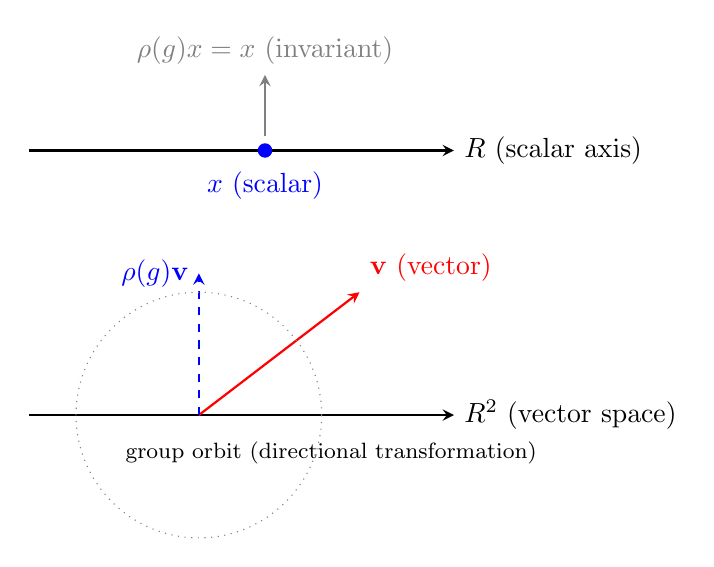
\begin{tikzpicture}[scale=1.2,>=stealth]
    \draw[->, thick] (0,0) -- (4.5,0) node[right] {$\mathbb{R}$ (scalar axis)};
    \filldraw[blue] (2.5,0) circle (2pt) node[below=4pt] {$x$ (scalar)};
    \draw[->, gray, thick] (2.5,0.15) -- (2.5,0.8) node[above] {$\rho(g)x = x$ (invariant)};

    \draw[->, thick] (0,-2.8) -- (4.5,-2.8) node[right] {$\mathbb{R}^2$ (vector space)};
    \draw[->, red, thick] (1.8,-2.8) -- (3.5,-1.5) node[above right] {$\mathbf{v}$ (vector)};
    \draw[->, blue, thick, dashed] (1.8,-2.8) -- (1.8,-1.3) node[left] {$\rho(g)\mathbf{v}$};
    \draw[gray, dotted] (1.8,-2.8) circle (1.3);
    \node[font=\footnotesize] at (3.2,-3.2) {group orbit (directional transformation)};
\end{tikzpicture}
\caption{The difference between scalars and vectors under a group action: a scalar is invariant under the group action (trivial representation, participating only in scaling); a vector changes its direction along the group orbit (non-trivial representation, participating in the three transformations of translation, scaling and rotation).}
\label{fig:scalar_vector_group_action}
\end{figure}

\begin{table}[htbp]
    \centering
    \caption{Correspondence between vector types, symmetry groups and directional structures}
    \label{tab:vector_types}
    \begin{tabular}{>{\centering\arraybackslash}p{2.2cm}>{\centering\arraybackslash}p{2cm}>{\centering\arraybackslash}p{2.5cm}>{\centering\arraybackslash}p{3cm}>{\centering\arraybackslash}p{2.5cm}}
        \toprule
        Vector type & Scalar field & Symmetry centre & Directional structure & Symmetry group \\
        \midrule
        Integer vector & $\mathbb{Z}$ & $0$ & Translation direction & $C_2$ (additive reflection) \\
        Rational vector & $\mathbb{Q}$ & $1$ & Proportional direction & $\mathbb{G}_m$ (multiplicative scaling reflection) \\
        Real vector & $\mathbb{R}$ & $0,1$ & Translation + proportion & $\mathbb{R}^+$ (continuous direction) \\
        Complex vector & $\mathbb{C}$ & $i$ & Rotation direction & $U(1)$ (taking the inverse) \\
        Quaternion vector & $\mathbb{H}$ & $i,j,k$ & Three-dimensional rotation & $SU(2)$ (non-commutative rotation) \\
        \bottomrule
    \end{tabular}
\end{table}
\section{\texorpdfstring{Basic operations in a vector space: translation, scaling and rotation}{Basic operations in a vector space: translation, scaling and rotation}}

\begin{definition}[Vector addition---translation]\label{def:vector_addition_translation}
Let $\mathbf{u} = (u_1,\dots,u_n)$, $\mathbf{v} = (v_1,\dots,v_n) \in \mathbb{R}^n$. Define \textbf{vector addition} (the translation operation):
\[\mathbf{u} + \mathbf{v} = (u_1+v_1, \dots, u_n+v_n).\]
This is the componentwise generalisation of the addition operation of the `Number Systems' chapter to a vector space, and also the vector realisation of the translation transformation of the `Operations and Periodicity' chapter. In addition, define the \textbf{zero vector} $\mathbf{0} = (0,\dots,0)$ (corresponding to the additive symmetry centre $0$), and the \textbf{negative vector} $-\mathbf{u} = (-u_1,\dots,-u_n)$ (corresponding to the additive inverse, that is, translation in the reverse direction).
\end{definition}

\begin{definition}[Scalar multiplication---scaling]\label{def:scalar_multiplication_scaling}
Let $\mathbf{u} \in \mathbb{R}^n$, $\alpha \in \mathbb{R}$. Define \textbf{scalar multiplication} (the scaling operation):
\[\alpha \mathbf{u} = (\alpha u_1, \dots, \alpha u_n).\]
This is the scalar-vector action of the multiplication operation of the `Number Systems' chapter on a vector space, and also the vector realisation of the scaling transformation of the `Operations and Periodicity' chapter. When $\alpha > 1$ it enlarges, when $0 < \alpha < 1$ it shrinks, when $\alpha = 1$ it leaves the vector unchanged ($1$ is the symmetry centre of the proportional direction), and when $\alpha = -1$ it reverses the vector.
\end{definition}

\begin{definition}[Outer product and complex multiplication---rotation]\label{def:outer_product_rotation}
The rotation operation has two equivalent realisations, according to the dimension of the space:
\begin{enumerate}[label=(\roman*)]
    \item \textbf{Outer product} (in $\mathbb{R}^3$): let $\mathbf{a}, \mathbf{b} \in \mathbb{R}^3$. Their \textbf{outer product} (cross product) $\mathbf{a} \times \mathbf{b}$ is a vector whose direction is perpendicular to the plane spanned by $\mathbf{a}$ and $\mathbf{b}$ (determined by the right-hand rule), and whose modulus is $\|\mathbf{a}\| \|\mathbf{b}\| \sin\theta$.
    \item \textbf{Complex multiplication} (in $\mathbb{R}^2 \cong \mathbb{C}$): let $z_1 = r_1 e^{i\alpha}, z_2 = r_2 e^{i\beta} \in \mathbb{C}$. Their product $z_1 z_2 = r_1 r_2 e^{i(\alpha+\beta)}$ adds the arguments of the two vectors and multiplies their moduli.
\end{enumerate}
The outer product and complex multiplication are the vector realisations of the rotation transformation of the `Operations and Periodicity' chapter.
\end{definition}

\begin{proposition}[The group structure of vector addition---the algebraic basis of translation]\label{prop:vector_additive_group}
Under vector addition, $\mathbb{R}^n$ forms a commutative group, with the zero vector as identity element and the negative vector as inverse element. This group is isomorphic to the direct product of $n$ additive groups of the real numbers. This is the direct realisation in a vector space of the additive reflection symmetry of the `Operations and Periodicity' chapter: the symmetry centre is $\mathbf{0}$, and the involution $\sigma_{\mathbf{0}}(\mathbf{u}) = -\mathbf{u}$ is an additive reflection automorphism of $\mathbb{R}^n$, generating a $C_2$ automorphism group.
\end{proposition}

\begin{proof}
Verify the group axioms: the associativity and commutativity of addition are inherited directly from the corresponding properties of real addition; the zero vector satisfies $\mathbf{u} + \mathbf{0} = \mathbf{u}$; and $\mathbf{u} + (-\mathbf{u}) = \mathbf{0}$. Hence $(\mathbb{R}^n, +)$ is a commutative group. The involution $\sigma_{\mathbf{0}}(\mathbf{u}) = -\mathbf{u}$ satisfies $\sigma_{\mathbf{0}} \circ \sigma_{\mathbf{0}} = \operatorname{id}$, and is an additive reflection with $\mathbf{0}$ as its unique fixed point. Since $\sigma_{\mathbf{0}} \neq \operatorname{id}$ and $\sigma_{\mathbf{0}}^2 = \operatorname{id}$, the group it generates is $C_2$.
\end{proof}

\begin{proposition}[The linearity of scalar multiplication---the algebraic basis of scaling]\label{prop:scalar_multiplication}
Scalar multiplication satisfies the following properties:
\begin{enumerate}[label=(\roman*)]
    \item $\alpha(\mathbf{u} + \mathbf{v}) = \alpha\mathbf{u} + \alpha\mathbf{v}$;
    \item $(\alpha + \beta)\mathbf{u} = \alpha\mathbf{u} + \beta\mathbf{u}$;
    \item $\alpha(\beta\mathbf{u}) = (\alpha\beta)\mathbf{u}$;
    \item $1 \cdot \mathbf{u} = \mathbf{u}$, where $1$ is the multiplicative identity, that is, the symmetry centre of the proportional direction.
\end{enumerate}
Scalar multiplication changes only the modulus of a vector and not its direction (except for reversal), and is the algebraic realisation of the \textbf{proportional scaling operation}.
\end{proposition}

\begin{proof}
Let $\mathbf{u} = (u_1,\dots,u_n)$, $\mathbf{v} = (v_1,\dots,v_n)$. (i) The $i$-th component of the left-hand side is $\alpha(u_i + v_i)$, and the $i$-th component of the right-hand side is $\alpha u_i + \alpha v_i$; the two are equal by the distributive law of the real numbers. (ii) The $i$-th component of the left-hand side is $(\alpha+\beta)u_i$, and that of the right-hand side is $\alpha u_i + \beta u_i$; they are equal by the distributive law of the real numbers. (iii) The left-hand side is $\alpha(\beta u_i) = (\alpha\beta)u_i$, and the right-hand side is $(\alpha\beta)u_i$; they are equal by the associativity of real multiplication. (iv) $1 \cdot u_i = u_i$, hence $1\cdot\mathbf{u} = \mathbf{u}$---the scalar $1$ is the identity of the multiplicative group (the scaling centre), and acting on a vector it changes neither its direction nor its magnitude. When $\alpha = 0$, $0\cdot u_i = 0$, hence $0\cdot\mathbf{u} = \mathbf{0}$: the zero scalar contracts any vector to the additive symmetry centre $\mathbf{0}$.
\end{proof}

\section{\texorpdfstring{Similarity: a pure measure of directional relations}{Similarity: a pure measure of directional relations}}

\begin{definition}[The computational origin of similarity]\label{def:similarity_root}
The similarity of this chapter is defined on $\mathbb{R}^2\cong\mathbb{C}$ (a single argument is required). Every similarity---whatever its angle type (difference angle, sum angle, double angle, half angle)---is in essence a scalar obtained by performing some algebraic operation on the arguments of two vectors and then taking the cosine or the sine. The sole source of information for a similarity is \textbf{the arguments of the two vectors} ($\alpha$ and $\beta$). The cosine series measures the \textbf{projection onto the real axis} after the operation on the arguments (an even function, insensitive to reversal of direction), whilst the sine series measures the \textbf{projection onto the imaginary axis} (an odd function, which changes sign when the direction is reversed).

In other words, the \textbf{entire diversity} of the similarity spectrum comes only from the different algebraic operations performed on the pair of arguments $(\alpha, \beta)$ ($\alpha - \beta$, $\alpha + \beta$, $2(\alpha - \beta)$, $2(\alpha + \beta)$, $(\alpha - \beta)/2$, $(\alpha + \beta)/2$). Beyond this, no further information is needed. The 12 basic similarities defined in this chapter all take this as their origin.
\end{definition}

\begin{lemma}[Generation of the 12 similarities]\label{lem:similarity_generation}
The 12 similarities are generated by the Cartesian product of the following three binary choices:
\[
\{\text{difference angle}, \text{sum angle}\} \times \{\text{basic}, \text{double angle}, \text{half angle}\} \times \{\text{cosine}, \text{sine}\} = 12.
\]
These three binary choices correspond respectively to three classes of operational duality:
\begin{enumerate}[label=(\roman*)]
    \item \textbf{Difference angle/sum angle} corresponds to \textbf{subtraction and addition} (translation direction, symmetry centre $c=0$): the difference angle (the signed difference $\alpha - \beta$) is the realisation of subtraction on the arguments, and the sum angle $\phi = \alpha + \beta$ is the realisation of addition on the arguments.
    \item \textbf{Double angle/half angle} corresponds to \textbf{powers and roots} (rotation direction, symmetry centre $c=i$): the double angle $2\theta$ is the power operation on the argument (rotating twice), and the half angle $\theta/2$ is the root operation on the argument (dividing the rotation equally).
    \item \textbf{Cosine/sine} corresponds to \textbf{real and imaginary parts} (projection and rotation): the cosine is the projection of the argument onto the real axis, and the sine is the projection of the argument onto the imaginary axis.
\end{enumerate}
Therefore the 12 similarities are generated by the Cartesian product of the operational duality.
\end{lemma}

\begin{proof}
The essence of similarity is to perform \textbf{a single algebraic operation} on the two arguments and then take a trigonometric function (Definition \ref{def:similarity_root}). A single algebraic operation has only three basic types: subtraction (difference angle), addition (sum angle), and \textbf{powers} of these two operations. When the exponent is $1$ it gives the basic angle ($\theta$ or $\phi$), when the exponent is $2$ it gives the double angle ($2\theta$ or $2\phi$), and when the exponent is $\frac{1}{2}$ it gives the half angle ($\theta/2$ or $\phi/2$). Operations with exponents exceeding $2$ (such as the triple angle $3\theta$) can be decomposed into composites of double and basic angles ($3\theta = 2\theta + \theta$), and hence do not fall within the scope of `basic similarities'---they can be obtained from the basic similarities by algebraic combination. Similarly, negative integer exponents or fractional exponents other than $\frac{1}{2}$ can also be decomposed into composites of the basic operations. Hence the $6$ basic angle operations $\{\theta, \phi, 2\theta, 2\phi, \theta/2, \phi/2\}$ are complete. Taking the cosine or the sine of each angle operation yields $6 \times 2 = 12$ basic similarities. The correspondence between the three binary choices and the operational duality is given directly by the definition.
\end{proof}

\begin{definition}[The essence of similarity]\label{def:similarity_essence}
Similarity is the core tool for describing the directional relation between two vectors. Its essential characteristic is that it \textbf{depends only on the arguments of the two vectors} and is completely independent of their moduli. The signed difference angle $\alpha - \beta$ measures the rotation angle required to rotate the direction of $\mathbf{b}$ to the direction of $\mathbf{a}$, and its absolute value is the included angle $\theta$ of the two vectors; the sum angle $\phi = \alpha + \beta$ measures the composition of the two directions in the rotation group.
\end{definition}

\subsection{\texorpdfstring{Difference-angle similarity}{Difference-angle similarity}}

\begin{definition}[Basic difference-angle similarity]\label{def:basic_diff_similarity}
Let $\mathbf{a}, \mathbf{b} \in \mathbb{R}^2\cong\mathbb{C}$ be non-zero vectors with arguments $\alpha$ and $\beta$ respectively. Following the unified convention of the `Scalars and Vectors' chapter, the \textbf{included angle} between two vector directions is always taken to be $\theta=\lvert\alpha-\beta\rvert\in[0,\pi]$; the signed quantity $\alpha-\beta$ is called the \textbf{difference angle} and is used only for the sign of the sine-family similarity. Define:
\begin{align*}
\operatorname{cosine}(\mathbf{a}, \mathbf{b}) &= \cos(\alpha - \beta) = \cos\theta \quad (\text{directional similarity}), \\
\operatorname{sine}(\mathbf{a}, \mathbf{b}) &= \sin(\alpha - \beta) \quad (\text{perpendicular similarity}).
\end{align*}
\end{definition}

\begin{proposition}[Properties of the basic difference-angle similarity]\label{prop:basic_diff_similarity_properties}
Let $\theta = \lvert\alpha-\beta\rvert \in [0, \pi]$ be the included angle of the two vectors. The directional similarity $\operatorname{cosine}$ and the perpendicular similarity $\operatorname{sine}$ satisfy:
\begin{enumerate}[label=(\roman*)]
    \item $\operatorname{cosine}(\mathbf{a}, \mathbf{b})$ measures the `agreement' of the two vectors along the translation direction: it attains its maximum $1$ when $\theta=0$ (exactly codirectional), and its minimum $-1$ when $\theta=\pi$ (exactly antidirectional).
    \item $\lvert\operatorname{sine}(\mathbf{a}, \mathbf{b})\rvert$ measures the `orthogonality' of the two vectors along the rotation direction: it attains its maximum $1$ when $\theta=\pi/2$ (exactly orthogonal).
    \item The two satisfy the identity: $\operatorname{cosine}^2 + \operatorname{sine}^2 = 1$.
\end{enumerate}
\end{proposition}

\begin{proof}
(i) follows directly from the monotonicity of the cosine function on $[0,\pi]$. (ii) follows from the identity $\operatorname{cosine}^2+\operatorname{sine}^2=1$ of (iii): $\lvert\operatorname{sine}\rvert$ attains its maximum $1$ at $\operatorname{cosine}=0$, that is, at $\theta=\pi/2$. (iii) is a direct consequence of the trigonometric identity $\cos^2\theta + \sin^2\theta = 1$.
\end{proof}

\begin{definition}[Double-angle difference-angle similarity]\label{def:double_diff_similarity}
The \textbf{axial similarity} and the \textbf{slope similarity} of the vectors $\mathbf{a}, \mathbf{b}$ are defined as:
\begin{align*}
\operatorname{cosine}_2(\mathbf{a}, \mathbf{b}) &= \cos 2(\alpha - \beta) = \cos 2\theta, \\
\operatorname{sine}_2(\mathbf{a}, \mathbf{b}) &= \sin 2(\alpha - \beta).
\end{align*}
\end{definition}

\begin{proposition}[Degeneracy detection by the double-angle difference-angle similarity]\label{prop:double_diff_degeneracy}
Let $\theta \in [0,\pi]$. The double-angle difference-angle similarity is used to detect degenerate states of direction:
\begin{enumerate}[label=(\roman*)]
    \item $\operatorname{cosine}_2 = 1$ if and only if $\theta = 0$ or $\pi$ (the two vectors are codirectional or antidirectional).
    \item $\operatorname{cosine}_2 = -1$ if and only if $\theta = \pi/2$ (the two vectors are orthogonal).
    \item $\lvert\operatorname{sine}_2\rvert = 1$ if and only if $\theta = \pi/4$ or $3\pi/4$ (the two directions are balanced or nearly opposite).
\end{enumerate}
\end{proposition}

\begin{proof}
Verify each critical value directly from $\cos 2\theta = 2\cos^2\theta - 1 = 1 - 2\sin^2\theta$. (i) $\cos 2\theta = 1 \iff 2\theta = 0 \text{ or } 2\pi \iff \theta = 0 \text{ or } \pi$ (since $\theta \in [0,\pi]$). (ii) $\cos 2\theta = -1 \iff 2\theta = \pi \iff \theta = \pi/2$. (iii) $\lvert\sin 2\theta\rvert = 1 \iff 2\theta = \pi/2 \text{ or } 3\pi/2 \iff \theta = \pi/4 \text{ or } 3\pi/4$ (since $\theta \in [0,\pi]$).
\end{proof}

\begin{definition}[Half-angle difference-angle similarity]\label{def:half_diff_similarity}
The \textbf{sum-direction similarity} and the \textbf{difference-direction similarity} of the vectors $\mathbf{a}, \mathbf{b}$ are defined as:
\begin{align*}
\operatorname{cosine}_{1/2}(\mathbf{a}, \mathbf{b}) &= \cos\frac{\theta}{2}, \\
\operatorname{sine}_{1/2}(\mathbf{a}, \mathbf{b}) &= \sin\frac{\theta}{2}, \qquad \theta = \lvert\alpha-\beta\rvert \in [0,\pi].
\end{align*}
\end{definition}

\begin{remark}\label{rem:half_angle_sum_difference}
The half-angle similarity is closely related to the moduli of the vector sum and difference (see Proposition \ref{prop:sum_difference_half_angle}). Under the equal-modulus condition, the modulus of the vector sum is proportional to $\cos(\theta/2)$, and the modulus of the vector difference is proportional to $\sin(\theta/2)$.
\end{remark}

\subsection{\texorpdfstring{Sum-angle similarity}{Sum-angle similarity}}

\begin{definition}[Basic sum-angle similarity]\label{def:basic_sum_similarity}
The \textbf{resultant-direction similarity} and the \textbf{resultant-perpendicular similarity} of the vectors $\mathbf{a}, \mathbf{b}$ are defined as:
\begin{align*}
\operatorname{cosine}_+(\mathbf{a}, \mathbf{b}) &= \cos(\alpha + \beta) = \cos\phi, \\
\operatorname{sine}_+(\mathbf{a}, \mathbf{b}) &= \sin(\alpha + \beta) = \sin\phi.
\end{align*}
The sum-angle similarity takes the sum of the arguments of the two vectors, $\phi = \alpha + \beta$, as its independent variable, and describes the \textbf{absolute directional composition} relation of the two vectors. It cannot be reduced to a difference-angle similarity, and corresponds naturally to the directional composition of complex multiplication---the composition of rotations.
\end{definition}

\begin{remark}[The essential difference between the difference angle and the sum angle]\label{rem:diff_sum_distinction}
The difference-angle similarity measures the \textbf{relative direction between two vectors}---this is the `observer's' viewpoint: the observer stands on one vector and measures the extent to which the other deviates from it. The sum-angle similarity measures the \textbf{composition of two vectors as independent directions}---this is the `participant's' viewpoint: the two directions each rotate independently, and are then composed into a new direction.
\end{remark}

\begin{figure}[htbp]
    \centering
    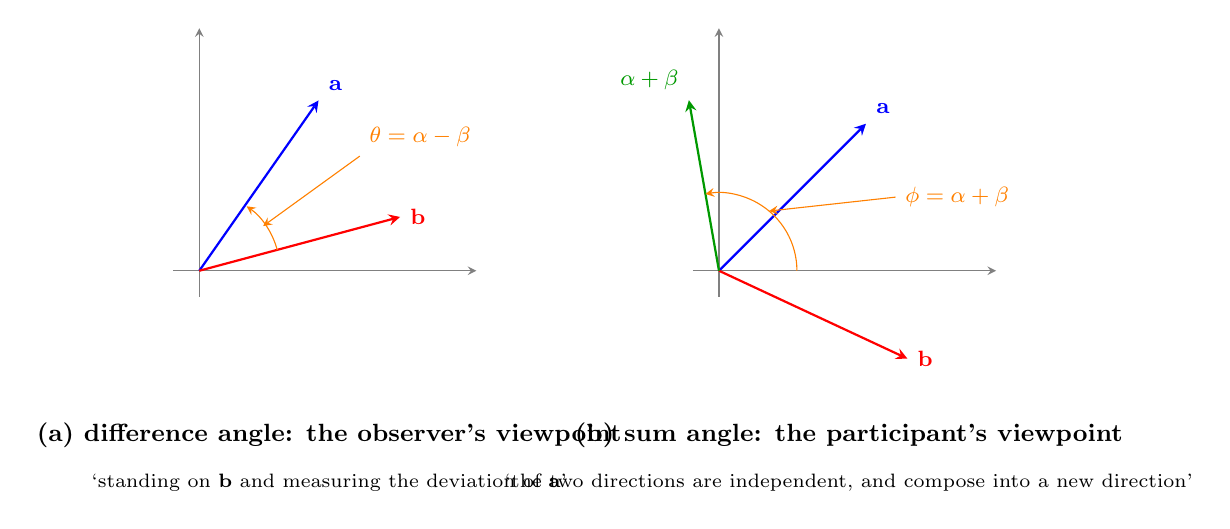
\begin{tikzpicture}[scale=1.1,>=stealth]

        \begin{scope}
            \draw[->, gray] (-0.3,0) -- (3.2,0);
            \draw[->, gray] (0,-0.3) -- (0,2.8);
            \draw[->, thick, blue] (0,0) -- (55:2.4) node[above right, font=\footnotesize] {$\mathbf{a}$};
            \draw[->, thick, red]  (0,0) -- (15:2.4) node[right, font=\footnotesize] {$\mathbf{b}$};
            \draw[->, orange] (0.9,0.24) arc (15:55:0.9);

            \node[orange, font=\footnotesize] (thlbl) at (2.55, 1.55) {$\theta=\lvert\alpha-\beta\rvert$};
            \draw[->, orange, thin] (thlbl.south west) -- (35:0.9);

            \node[font=\small\bfseries] at (1.5,-1.9)
                {(a) difference angle: the observer's viewpoint};
            \node[font=\scriptsize, align=center] at (1.5,-2.45)
                {`standing on $\mathbf{b}$ and measuring the deviation of $\mathbf{a}$'};
        \end{scope}

        \begin{scope}[xshift=6.0cm]
            \draw[->, gray] (-0.3,0) -- (3.2,0);
            \draw[->, gray] (0,-0.3) -- (0,2.8);
            \draw[->, thick, blue] (0,0) -- (45:2.4) node[above right, font=\footnotesize] {$\mathbf{a}$};
            \draw[->, thick, red]  (0,0) -- (-25:2.4) node[right, font=\footnotesize] {$\mathbf{b}$};
            \draw[->, thick, green!60!black] (0,0) -- (100:2.0)
                node[above left, font=\footnotesize] {$\alpha+\beta$};
            \draw[->, orange] (0.9,0) arc (0:100:0.9);

            \node[orange, font=\footnotesize] (phlbl) at (2.75, 0.85) {$\phi=\alpha+\beta$};
            \draw[->, orange, thin] (phlbl.west) -- (50:0.9);

            \node[font=\small\bfseries] at (1.5,-1.9)
                {(b) sum angle: the participant's viewpoint};
            \node[font=\scriptsize, align=center] at (1.5,-2.45)
                {`the two directions are independent, and compose into a new direction'};
        \end{scope}
    \end{tikzpicture}
    \caption{Comparison of the geometric viewpoints of the difference-angle similarity and the sum-angle similarity. (a) The difference angle $\theta=\lvert\alpha-\beta\rvert$ measures the relative deviation between two directions, and is the `observer's' viewpoint; (b) the sum angle $\phi=\alpha+\beta$ measures the total deflection of the composition of the two directions (the argument of the composed direction being $\alpha+\beta$), and is the `participant's' viewpoint. The two cannot be reduced to one another (Remark \ref{rem:diff_sum_distinction}).}
    \label{fig:diff_vs_sum_angle}
\end{figure}

\begin{definition}[Double-angle sum-angle similarity]\label{def:double_sum_similarity}
The \textbf{double-angle resultant-direction similarity} and the \textbf{double-angle resultant-perpendicular similarity} of the vectors $\mathbf{a}, \mathbf{b}$ are defined as:
\begin{align*}
\operatorname{cosine}_{2+}(\mathbf{a}, \mathbf{b}) &= \cos 2(\alpha + \beta) = \cos 2\phi, \\
\operatorname{sine}_{2+}(\mathbf{a}, \mathbf{b}) &= \sin 2(\alpha + \beta) = \sin 2\phi.
\end{align*}
\end{definition}

\begin{definition}[Half-angle sum-angle similarity]\label{def:half_sum_similarity}
The \textbf{half-angle resultant-direction similarity} and the \textbf{half-angle resultant-perpendicular similarity} of the vectors $\mathbf{a}, \mathbf{b}$ are defined as:
\begin{align*}
\operatorname{cosine}_{1/2+}(\mathbf{a}, \mathbf{b}) &= \cos\frac{\alpha + \beta}{2} = \cos\frac{\phi}{2}, \\
\operatorname{sine}_{1/2+}(\mathbf{a}, \mathbf{b}) &= \sin\frac{\alpha + \beta}{2} = \sin\frac{\phi}{2}.
\end{align*}
\end{definition}
\subsection{\texorpdfstring{Overview of the 12 basic similarities}{Overview of the 12 basic similarities}}

\begin{table}[htbp]
    \centering
    \caption{The spectrum of the 12 basic similarities}
    \label{tab:similarity_spectrum}
    \begin{tabular}{>{\centering\arraybackslash}p{2.2cm}>{\centering\arraybackslash}p{2cm}>{\centering\arraybackslash}p{3.5cm}>{\centering\arraybackslash}p{3.5cm}}
        \toprule
        Angle type & Level & Cosine similarity (cosine) & Sine similarity (sine) \\
        \midrule
        \multirow{3}*{\parbox{2.0cm}{\centering difference angle $\theta=\lvert\alpha-\beta\rvert$}}
        & Basic & $\cos\theta$ (directional similarity) & $\sin\theta$ (perpendicular similarity) \\
        & Double angle & $\cos 2\theta$ (axial similarity) & $\sin 2\theta$ (slope similarity) \\
        & Half angle & $\cos\frac{\theta}{2}$ (sum-direction similarity) & $\sin\frac{\theta}{2}$ (difference-direction similarity) \\
        \midrule
        \multirow{3}*{\parbox{2.0cm}{\centering sum angle $\phi=\alpha+\beta$}}
        & Basic & $\cos\phi$ (resultant-direction similarity) & $\sin\phi$ (resultant-perpendicular similarity) \\
        & Double angle & $\cos 2\phi$ (double-angle resultant-direction similarity) & $\sin 2\phi$ (double-angle resultant-perpendicular similarity) \\
        & Half angle & $\cos\frac{\phi}{2}$ (half-angle resultant-direction similarity) & $\sin\frac{\phi}{2}$ (half-angle resultant-perpendicular similarity) \\
        \bottomrule
    \end{tabular}
\end{table}

\begin{figure}[htbp]
    \centering
    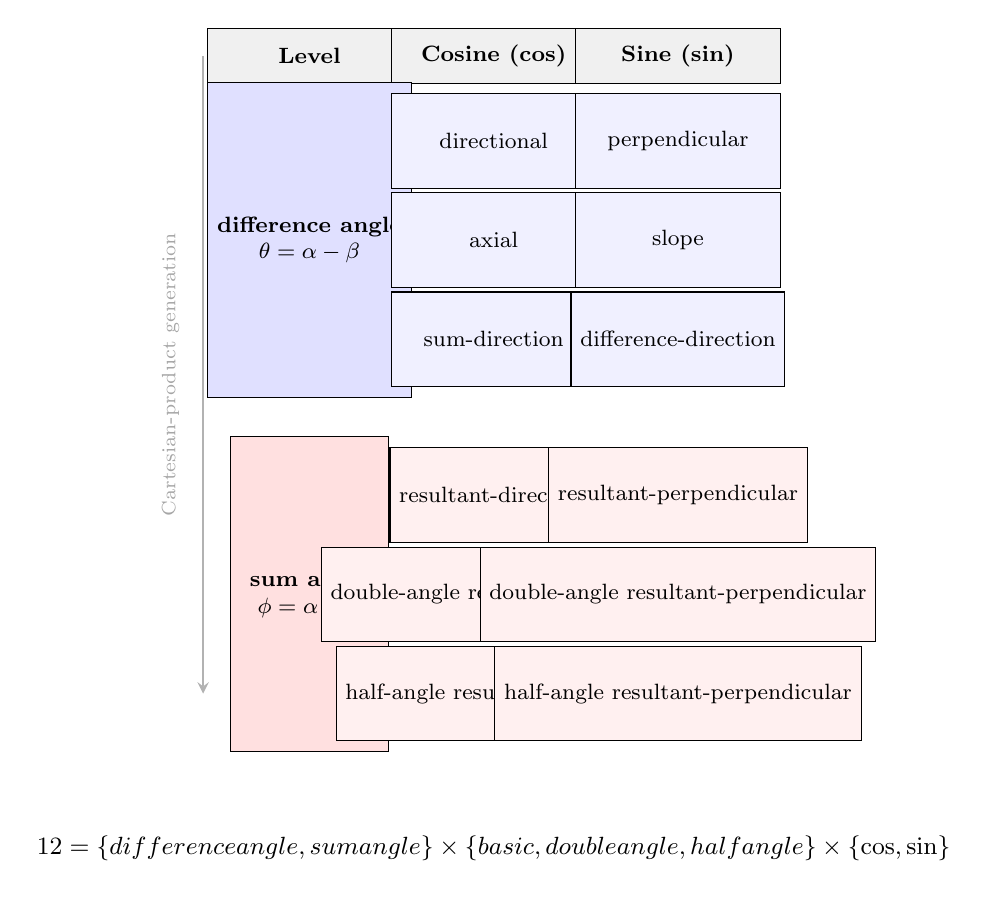
\begin{tikzpicture}[scale=0.9,>=stealth,
        cell/.style={draw, minimum width=2.6cm, minimum height=1.2cm,
                     align=center, font=\footnotesize},
        hdr/.style={draw, fill=gray!12, minimum width=2.6cm, minimum height=0.7cm,
                    align=center, font=\footnotesize\bfseries},
        rowlbl/.style={draw, fill=gray!8, minimum width=2.0cm, minimum height=4.0cm,
                       align=center, font=\footnotesize\bfseries}]

        \node[hdr] at (0, 3.0) {Level};
        \node[hdr] at (2.6, 3.0) {Cosine (cos)};
        \node[hdr] at (5.2, 3.0) {Sine (sin)};

        \node[rowlbl, fill=blue!12] at (0, 0.4)
            {difference angle\\ $\theta=\lvert\alpha-\beta\rvert$};

        \node[cell, fill=blue!6] at (2.6, 1.8) {directional};
        \node[cell, fill=blue!6] at (5.2, 1.8) {perpendicular};
        \node[cell, fill=blue!6] at (2.6, 0.4) {axial};
        \node[cell, fill=blue!6] at (5.2, 0.4) {slope};
        \node[cell, fill=blue!6] at (2.6,-1.0) {sum-direction};
        \node[cell, fill=blue!6] at (5.2,-1.0) {difference-direction};

        \node[rowlbl, fill=red!12] at (0, -4.6)
            {sum angle\\ $\phi=\alpha+\beta$};

        \node[cell, fill=red!6] at (2.6,-3.2) {resultant-direction};
        \node[cell, fill=red!6] at (5.2,-3.2) {resultant-perpendicular};
        \node[cell, fill=red!6] at (2.6,-4.6) {double-angle resultant-direction};
        \node[cell, fill=red!6] at (5.2,-4.6) {double-angle resultant-perpendicular};
        \node[cell, fill=red!6] at (2.6,-6.0) {half-angle resultant-direction};
        \node[cell, fill=red!6] at (5.2,-6.0) {half-angle resultant-perpendicular};

        \draw[->, gray!60, thick] (-1.5, 3.0) -- (-1.5, -6.0);
        \node[gray!70, font=\scriptsize, rotate=90, anchor=south] at (-1.7, -1.5)
            {Cartesian-product generation};

        \node[font=\small\bfseries, below=0.6cm] at (2.6,-7.2)
            {$12 = \{\text{difference angle},\text{sum angle}\}\times\{\text{basic},\text{double angle},\text{half angle}\}\times\{\cos,\sin\}$};
    \end{tikzpicture}
    \caption{The two-dimensional lattice spectrum of the 12 basic similarities (a schematic diagram of the generation rule). The horizontal binary choice is cosine/sine (projection onto the real/imaginary part), whilst the vertical one is the composite of difference angle/sum angle (subtraction/addition) with basic/double angle/half angle (powers). Each cell corresponds to one similarity, and the concrete formulae are given in the immediately adjacent Table \ref{tab:similarity_spectrum}; the point of this figure is to display explicitly the $2\times3\times2$ Cartesian-product generation structure (Lemma \ref{lem:similarity_generation}).}
    \label{fig:similarity_spectrum_grid}
\end{figure}

\begin{remark}[Complex exponential packaging and quaternion packaging]\label{rem:exponential_packaging}
The basic difference-angle cosine similarity and the basic difference-angle sine similarity can be unified as the complex exponential similarity
$\operatorname{Similarity}^{\mathbb C}(a,b)=e^{i(\alpha-\beta)}$;
the basic difference-angle cosine tendency and the signed sine tendency can be unified as the complex exponential tendency
$\operatorname{Tendency}^{\mathbb C}(a,b)=a\overline b$.
In the quaternion case one defines, by angle difference and angle sum, the difference-angle quaternion
$D_{\mathbb H}(p,q)=p\overline q/(|p||q|)$
and the sum-angle quaternion
$S_{\mathbb H}(p,q)=pq/(|p||q|)$,
which give three-dimensional rotation operators through the conjugation action. See Section \ref{sec:complex_quaternion_exponential_similarity} for details.
\end{remark}
\section{\texorpdfstring{Tendency: a composite measure of direction and scale}{Tendency: a composite measure of direction and scale}}

\begin{definition}[The computational origin of tendency]\label{def:tendency_root}
Every tendency---whatever the type of similarity to which it corresponds---is in essence the product of the corresponding similarity and the moduli of the two vectors:
\[
\text{tendency} = \text{similarity} \times \|\mathbf{a}\| \times \|\mathbf{b}\|.
\]
The information sources of a tendency are of two kinds: \textbf{the arguments of the two vectors} (supplying the similarity) and \textbf{the moduli of the two vectors} (supplying the scale). The similarity encodes a purely directional relation (depending only on the difference or the sum of the arguments), whilst the product of the moduli encodes scale information. The tendency synthesises the two into a single scalar, giving a complete measure of `directed scale'.
\end{definition}

\begin{proposition}[Similarity is the reduction of tendency]\label{prop:similarity_reduction}
Let $T(\mathbf{a},\mathbf{b})$ be a tendency and let $S(\mathbf{a},\mathbf{b})$ be the corresponding similarity. Then
\[
S(\mathbf{a},\mathbf{b}) = \frac{T(\mathbf{a},\mathbf{b})}{\|\mathbf{a}\| \|\mathbf{b}\|}.
\]
That is, the similarity is the reduction of the tendency after normalisation of the moduli. The similarity retains only directional information, whilst the tendency retains both directional information and scale information.
\end{proposition}

\begin{proof}
From the definition of tendency, $T(\mathbf{a},\mathbf{b}) = \|\mathbf{a}\| \|\mathbf{b}\| \cdot S(\mathbf{a},\mathbf{b})$; dividing both sides by the non-zero quantity $\|\mathbf{a}\| \|\mathbf{b}\|$ gives the result.
\end{proof}

\begin{corollary}[Completeness of the 12 tendencies]\label{cor:tendency_completeness}
The 12 tendencies are generated by a one-to-one correspondence between the 12 similarities and the product of moduli $\|\mathbf{a}\|\|\mathbf{b}\|$. The completeness of the similarities (Lemma \ref{lem:similarity_generation}) directly guarantees the completeness of the tendencies.
\end{corollary}

\begin{proof}
By the definition of tendency (Definition \ref{def:tendency_root}), each similarity $S$ corresponds uniquely to a tendency $T = \|\mathbf{a}\|\|\mathbf{b}\| \cdot S$. The map $S \mapsto T$ is a bijection (since $\|\mathbf{a}\|\|\mathbf{b}\| \neq 0$). Lemma \ref{lem:similarity_generation} guarantees that the set of similarities has exactly 12 elements, so the set of tendencies likewise has exactly 12 elements.
\end{proof}

\begin{definition}[Tendency]\label{def:tendency}
Let $\mathbf{a}, \mathbf{b} \in \mathbb{R}^2$ be non-zero vectors. For any kind of similarity $S(\mathbf{a}, \mathbf{b})$, the corresponding \textbf{tendency} $T(\mathbf{a}, \mathbf{b})$ is defined as the product of that similarity and the moduli of the two vectors:
\[
T(\mathbf{a}, \mathbf{b}) = \|\mathbf{a}\| \|\mathbf{b}\| \cdot S(\mathbf{a}, \mathbf{b}).
\]
If one of the two vectors is the zero vector, the tendency is zero---this corresponds to the degeneration of the scaling factor to the additive symmetry centre $0$.
\end{definition}

\subsection{\texorpdfstring{Difference-angle tendency}{Difference-angle tendency}}

\begin{definition}[Basic difference-angle tendency]\label{def:basic_diff_tendency}
The tendency corresponding to the basic difference-angle similarity is:
\begin{align*}
\operatorname{cosine\_tendency}(\mathbf{a}, \mathbf{b}) &= \|\mathbf{a}\| \|\mathbf{b}\| \cos\theta = \mathbf{a} \cdot \mathbf{b}, \\
\operatorname{sine\_tendency}(\mathbf{a}, \mathbf{b}) &= \|\mathbf{a}\| \|\mathbf{b}\| \sin(\alpha-\beta), \\
\lvert\operatorname{sine\_tendency}(\mathbf{a}, \mathbf{b})\rvert &= \|\mathbf{a}\| \|\mathbf{b}\| \sin\theta = \|\mathbf{a} \times \mathbf{b}\| \quad (\text{in } \mathbb{R}^3 \text{, where } \theta \text{ is the included angle}).
\end{align*}
The cosine tendency is the inner product, a scaled projection measure along the translation direction; the absolute value of the sine tendency is the modulus of the outer product, a scaled directed-area measure along the rotation direction.
\end{definition}

\begin{proposition}[The correspondence between the basic difference-angle tendency and the vector operations]\label{prop:diff_tendency_relations}
The basic difference-angle tendency has the following exact correspondences with the basic vector operations:
\begin{enumerate}[label=(\roman*)]
    \item \textbf{The cosine tendency is the inner product}: $\operatorname{cosine\_tendency}(\mathbf{a}, \mathbf{b}) = \mathbf{a} \cdot \mathbf{b}$. The inner product is the projection measure along the translation direction.
    \item \textbf{The absolute value of the sine tendency is the modulus of the outer product}: $\lvert\operatorname{sine\_tendency}(\mathbf{a}, \mathbf{b})\rvert = \|\mathbf{a} \times \mathbf{b}\|$. The modulus of the outer product is the directed-area measure along the rotation direction.
\end{enumerate}
\end{proposition}

\begin{proof}
(i) follows directly from the geometric definition of the inner product $\mathbf{a} \cdot \mathbf{b} = \|\mathbf{a}\| \|\mathbf{b}\| \cos\theta$ and the definition of the cosine tendency. (ii) follows directly from the geometric definition of the outer product $\|\mathbf{a} \times \mathbf{b}\| = \|\mathbf{a}\| \|\mathbf{b}\| \sin\theta$ (with $\theta$ the included angle of the two vectors) and the definition of the sine tendency, on taking absolute values of both sides.
\end{proof}

\begin{definition}[Double-angle difference-angle tendency]\label{def:double_diff_tendency}
The double-angle difference-angle tendency is obtained from the double-angle difference-angle similarity and the product of the moduli:
\begin{align*}
\operatorname{cosine\_tendency}_2(\mathbf{a}, \mathbf{b}) &= \|\mathbf{a}\| \|\mathbf{b}\| \cos 2\theta, \\
\operatorname{sine\_tendency}_2(\mathbf{a}, \mathbf{b}) &= \|\mathbf{a}\| \|\mathbf{b}\| \sin 2\theta.
\end{align*}
\end{definition}

\begin{definition}[Half-angle difference-angle tendency]\label{def:half_diff_tendency}
The half-angle difference-angle tendency is obtained from the half-angle difference-angle similarity and the product of the moduli:
\begin{align*}
\operatorname{cosine\_tendency}_{1/2}(\mathbf{a}, \mathbf{b}) &= \|\mathbf{a}\| \|\mathbf{b}\| \cos\frac{\theta}{2}, \\
\operatorname{sine\_tendency}_{1/2}(\mathbf{a}, \mathbf{b}) &= \|\mathbf{a}\| \|\mathbf{b}\| \sin\frac{\theta}{2}.
\end{align*}
\end{definition}

\subsection{\texorpdfstring{Sum-angle tendency}{Sum-angle tendency}}

\begin{definition}[Basic sum-angle tendency]\label{def:basic_sum_tendency}
The tendency corresponding to the basic sum-angle similarity is:
\begin{align*}
\operatorname{cosine\_tendency}_+(\mathbf{a}, \mathbf{b}) &= \|\mathbf{a}\| \|\mathbf{b}\| \cos(\alpha + \beta), \\
\operatorname{sine\_tendency}_+(\mathbf{a}, \mathbf{b}) &= \|\mathbf{a}\| \|\mathbf{b}\| \sin(\alpha + \beta).
\end{align*}
\end{definition}

\begin{definition}[Double-angle sum-angle tendency]\label{def:double_sum_tendency}
The double-angle sum-angle tendency is obtained from the double-angle sum-angle similarity and the product of the moduli:
\begin{align*}
\operatorname{cosine\_tendency}_{2+}(\mathbf{a}, \mathbf{b}) &= \|\mathbf{a}\| \|\mathbf{b}\| \cos 2(\alpha + \beta), \\
\operatorname{sine\_tendency}_{2+}(\mathbf{a}, \mathbf{b}) &= \|\mathbf{a}\| \|\mathbf{b}\| \sin 2(\alpha + \beta).
\end{align*}
\end{definition}

\begin{definition}[Half-angle sum-angle tendency]\label{def:half_sum_tendency}
The half-angle sum-angle tendency is obtained from the half-angle sum-angle similarity and the product of the moduli:
\begin{align*}
\operatorname{cosine\_tendency}_{1/2+}(\mathbf{a}, \mathbf{b}) &= \|\mathbf{a}\| \|\mathbf{b}\| \cos\frac{\alpha + \beta}{2}, \\
\operatorname{sine\_tendency}_{1/2+}(\mathbf{a}, \mathbf{b}) &= \|\mathbf{a}\| \|\mathbf{b}\| \sin\frac{\alpha + \beta}{2}.
\end{align*}
\end{definition}

\subsection{\texorpdfstring{Overview of the 12 tendencies}{Overview of the 12 tendencies}}

\begin{table}[htbp]
    \centering
    \caption{The correspondence between the 12 tendencies and the vector operations}
    \label{tab:tendency_spectrum}
    \begin{tabularx}{\textwidth}{>{\centering\arraybackslash}p{2.4cm}
                                >{\centering\arraybackslash}p{1.4cm}
                                >{\centering\arraybackslash}X
                                >{\centering\arraybackslash}X}
        \toprule
        Angle type & Level & Cosine tendency (cosine tendency) & Sine tendency (sine tendency) \\
        \midrule
        \multirow{3}*{\parbox{2.0cm}{\centering difference angle $\theta=\lvert\alpha-\beta\rvert$}}
        & Basic & $\mathbf{a} \cdot \mathbf{b}$ (inner product) & $\|\mathbf{a}\| \|\mathbf{b}\| \sin(\alpha-\beta)$ (signed; its absolute value is the modulus of the outer product) \\
        & Double angle & $\|\mathbf{a}\| \|\mathbf{b}\| \cos 2\theta$ & $\|\mathbf{a}\| \|\mathbf{b}\| \sin 2\theta$ (signed) \\
        & Half angle & $\|\mathbf{a}\| \|\mathbf{b}\| \cos\frac{\theta}{2}$ & $\|\mathbf{a}\| \|\mathbf{b}\| \sin\frac{\theta}{2}$ \\
        \midrule
        \multirow{3}*{\parbox{2.0cm}{\centering sum angle $\phi=\alpha+\beta$}}
        & Basic & $\operatorname{Re}(z_1 z_2)$ & $\operatorname{Im}(z_1 z_2)$ \\
        & Double angle & $\|\mathbf{a}\| \|\mathbf{b}\| \cos 2\phi$ & $\|\mathbf{a}\| \|\mathbf{b}\| \sin 2\phi$ \\
        & Half angle & $\|\mathbf{a}\| \|\mathbf{b}\| \cos\frac{\phi}{2}$ & $\|\mathbf{a}\| \|\mathbf{b}\| \sin\frac{\phi}{2}$ \\
        \bottomrule
    \end{tabularx}
\end{table}

\section{\texorpdfstring{Inner and outer products: the geometric realisation of the cosine and sine tendencies}{Inner and outer products: the geometric realisation of the cosine and sine tendencies}}

\begin{property}[Basic properties of the inner product]\label{prop:inner_product_properties}
Let $\mathbf{a}, \mathbf{b}, \mathbf{c} \in \mathbb{R}^n$, $\alpha, \beta \in \mathbb{R}$. The inner product satisfies:
\begin{enumerate}[label=(\roman*)]
    \item \textbf{Symmetry}: $\mathbf{a} \cdot \mathbf{b} = \mathbf{b} \cdot \mathbf{a}$;
    \item \textbf{Bilinearity}: $(\alpha\mathbf{a} + \beta\mathbf{b}) \cdot \mathbf{c} = \alpha(\mathbf{a}\cdot\mathbf{c}) + \beta(\mathbf{b}\cdot\mathbf{c})$;
    \item \textbf{Positive definiteness}: $\mathbf{a} \cdot \mathbf{a} \ge 0$, and $\mathbf{a}\cdot\mathbf{a} = 0 \iff \mathbf{a} = \mathbf{0}$.
\end{enumerate}
\end{property}

\begin{property}[Basic properties of the outer product]\label{prop:outer_product_properties}
Let $\mathbf{a}, \mathbf{b}, \mathbf{c} \in \mathbb{R}^3$, $\alpha, \beta \in \mathbb{R}$. The outer product satisfies:
\begin{enumerate}[label=(\roman*)]
    \item \textbf{Anti-commutativity}: $\mathbf{a} \times \mathbf{b} = -\mathbf{b} \times \mathbf{a}$;
    \item \textbf{Bilinearity}: $(\alpha\mathbf{a} + \beta\mathbf{b}) \times \mathbf{c} = \alpha(\mathbf{a}\times\mathbf{c}) + \beta(\mathbf{b}\times\mathbf{c})$;
    \item \textbf{The Jacobi identity}: $\mathbf{a} \times (\mathbf{b} \times \mathbf{c}) + \mathbf{b} \times (\mathbf{c} \times \mathbf{a}) + \mathbf{c} \times (\mathbf{a} \times \mathbf{b}) = \mathbf{0}$.
\end{enumerate}
\end{property}

\begin{proposition}[The cosine tendency is an orthogonal-group invariant---the vector realisation of the conservation theme]\label{prop:cosine_scalar}
Let $G = O(n)$ be the orthogonal group on $\mathbb{R}^n$. For any $R \in O(n)$ and any non-zero vectors $\mathbf{a}, \mathbf{b} \in \mathbb{R}^n$, the cosine similarity and the cosine tendency are invariant under the group action:
\[\operatorname{cosine}(R\mathbf{a}, R\mathbf{b}) = \operatorname{cosine}(\mathbf{a}, \mathbf{b}), \quad (R\mathbf{a}) \cdot (R\mathbf{b}) = \mathbf{a} \cdot \mathbf{b}.\]

The invariance of the inner product (cosine tendency) under the orthogonal group $O(n)$ is the core fact of the conservation theme of this chapter: after an arbitrary orthogonal transformation (rotation or reflection) of two vectors, their projection measure along the translation direction is strictly conserved.
\end{proposition}

\begin{proof}
Let the matrix entries of $R$ be $R_{ij}$, satisfying $R^{\mathsf T}R = I$, that is, $\sum_k R_{ki}R_{kj} = \delta_{ij}$. Compute the inner product:
\begin{align*}
(R\mathbf{a}) \cdot (R\mathbf{b})
&= \sum_i \left( \sum_j R_{ij} a_j \right) \left( \sum_k R_{ik} b_k \right) \\
&= \sum_{j,k} a_j b_k \left( \sum_i R_{ij}R_{ik} \right) \\
&= \sum_{j,k} a_j b_k \delta_{jk}
= \mathbf{a} \cdot \mathbf{b}.
\end{align*}
At the same time, an orthogonal transformation preserves the modulus: $\|R\mathbf{a}\| = \|\mathbf{a}\|$, $\|R\mathbf{b}\| = \|\mathbf{b}\|$. Therefore
\[
\operatorname{cosine}(R\mathbf{a}, R\mathbf{b})
= \frac{R\mathbf{a} \cdot R\mathbf{b}}{\|R\mathbf{a}\| \|R\mathbf{b}\|}
= \frac{\mathbf{a} \cdot \mathbf{b}}{\|\mathbf{a}\| \|\mathbf{b}\|}
= \operatorname{cosine}(\mathbf{a}, \mathbf{b}).
\]
\end{proof}

\begin{proposition}[The absolute value of the sine tendency is invariant under pure rotations---the curl realisation of the conservation theme]\label{prop:sine_rotation}
Let $R \in SO(3)$ be a rotation of three-dimensional space. Then for any non-zero vectors $\mathbf{a},\mathbf{b} \in \mathbb{R}^3$ one has
\[\lvert\operatorname{sine}(R\mathbf{a}, R\mathbf{b})\rvert = \lvert\operatorname{sine}(\mathbf{a}, \mathbf{b})\rvert.\]

The absolute value of the sine tendency (the modulus of the outer product, the directed-area measure along the rotation direction) is strictly conserved under pure rotations $SO(3)$---this is the realisation, at the vector level, of the conservation law in the curl direction (conservation of angular momentum): rotation about an arbitrary axis does not change the \textbf{magnitude} of the directed area spanned by the two vectors; the direction of the directed area transforms in step with the rotation.
\end{proposition}

\begin{proof}
By the transformation property of the outer product under rotation, $(R\mathbf{a}) \times (R\mathbf{b}) = R(\mathbf{a} \times \mathbf{b})$. A rotation preserves the modulus, hence $\|(R\mathbf{a}) \times (R\mathbf{b})\| = \|R(\mathbf{a} \times \mathbf{b})\| = \|\mathbf{a} \times \mathbf{b}\|$. Also $\|R\mathbf{a}\| = \|\mathbf{a}\|$ and $\|R\mathbf{b}\| = \|\mathbf{b}\|$, hence $\lvert\operatorname{sine}(R\mathbf{a}, R\mathbf{b})\rvert = \|(R\mathbf{a}) \times (R\mathbf{b})\| / (\|R\mathbf{a}\| \|R\mathbf{b}\|) = \|\mathbf{a} \times \mathbf{b}\| / (\|\mathbf{a}\| \|\mathbf{b}\|) = \lvert\operatorname{sine}(\mathbf{a}, \mathbf{b})\rvert$, that is, $\lvert\operatorname{sine}\rvert$ is invariant under pure rotations.
\end{proof}

\section{\texorpdfstring{Vector sum, vector difference and the half-angle tendency}{Vector sum, vector difference and the half-angle tendency}}

\begin{proposition}[The vector sum and difference and the half-angle tendency]\label{prop:sum_difference_half_angle}
Let $\mathbf{a}, \mathbf{b} \in \mathbb{R}^n$ be non-zero vectors of equal modulus ($\|\mathbf{a}\| = \|\mathbf{b}\| = r>0$), and let $\theta \in [0,\pi]$ be the included angle of the two vectors. Then:
\begin{enumerate}[label=(\roman*)]
    \item the modulus of the vector sum $\mathbf{a} + \mathbf{b}$ is proportional to the half-angle cosine similarity: $\|\mathbf{a} + \mathbf{b}\| = 2r\cos\frac{\theta}{2}$.
    \item the modulus of the vector difference $\mathbf{a} - \mathbf{b}$ is proportional to the half-angle sine similarity: $\|\mathbf{a} - \mathbf{b}\| = 2r\sin\frac{\theta}{2}$.
\end{enumerate}
\end{proposition}

\begin{proof}
(i) By the parallelogram law,
\[\|\mathbf{a} + \mathbf{b}\|^2 = \|\mathbf{a}\|^2 + \|\mathbf{b}\|^2 + 2\mathbf{a}\cdot\mathbf{b} = 2r^2 + 2r^2\cos\theta = 2r^2(1 + \cos\theta).\]
Using the half-angle formula $1 + \cos\theta = 2\cos^2\frac{\theta}{2}$, we obtain $\|\mathbf{a} + \mathbf{b}\|^2 = 4r^2\cos^2\frac{\theta}{2}$. Since $\|\mathbf{a} + \mathbf{b}\| \ge 0$ and $\cos\frac{\theta}{2} \ge 0$ (because $\theta \in [0,\pi]$ implies $\frac{\theta}{2} \in [0,\frac{\pi}{2}]$), taking the square root gives the result.

(ii) Likewise,
\[\|\mathbf{a} - \mathbf{b}\|^2 = \|\mathbf{a}\|^2 + \|\mathbf{b}\|^2 - 2\mathbf{a}\cdot\mathbf{b} = 2r^2 - 2r^2\cos\theta = 2r^2(1 - \cos\theta).\]
Using $1 - \cos\theta = 2\sin^2\frac{\theta}{2}$, and noting that $\sin\frac{\theta}{2}\ge0$ because $\theta\in[0,\pi]$, taking the square root gives $\|\mathbf{a}-\mathbf{b}\|=2r\sin\frac{\theta}{2}$.
\end{proof}

\begin{figure}[htbp]
    \centering
    \begin{tikzpicture}[scale=1.0,>=stealth]

        \coordinate (O) at (0,0);
        \coordinate (A) at (55:2.4);
        \coordinate (B) at (15:2.4);
        \coordinate (S) at ($(A)+(B)$);

        \draw[->, thick, blue] (O) -- (A)
            node[above left, font=\footnotesize] {$\mathbf{a}$};
        \draw[->, thick, red]  (O) -- (B)
            node[below right, font=\footnotesize] {$\mathbf{b}$};

        \draw[orange, thick] (15:0.85) arc (15:55:0.85);
        \node[orange, font=\footnotesize] (theta) at (-1.3, 1.3) {$\theta$};
        \draw[orange, ->, thin] (theta.east) -- (25:0.85);

        \draw[gray, dashed, thick] (15:1.3) arc (15:35:1.3);
        \node[gray, font=\footnotesize] (thetahalf) at (4.0, -1.5) {$\theta/2$};
        \draw[gray, ->, thin] (thetahalf.north west) -- (25:1.3);

        \draw[->, thick, green!60!black] (O) -- (S);
        \draw[gray, dashed] (A) -- (S);
        \draw[gray, dashed] (B) -- (S);

        \node[green!60!black, font=\footnotesize, align=left] (sumlbl) at (3.1, 3.5)
            {$\|\mathbf{a}+\mathbf{b}\|=2r\cos\frac{\theta}{2}$};
        \draw[green!60!black, ->, thin] (sumlbl.south) -- (S);

        \draw[->, thick, magenta] (B) -- (A);

        \node[magenta, font=\footnotesize, align=left] (difflbl) at (-3.4, 2.4)
            {$\|\mathbf{a}-\mathbf{b}\|=2r\sin\frac{\theta}{2}$};
        \draw[magenta, ->, thin] (difflbl.east) -- ($(A)!0.5!(B)$);

        \node[font=\small\bfseries, align=center] at (1.8, -2.4)
            {when the moduli are equal, $\|\mathbf{a}\|=\|\mathbf{b}\|=r$, the half-angle formulae hold exactly};

    \end{tikzpicture}
    \caption{The geometric relation between the half-angle similarity and the vector sum/difference. Under the equal-modulus condition, the modulus of the vector sum is proportional to the half-angle cosine (sum-direction), and the modulus of the vector difference is proportional to the half-angle sine (difference-direction). The symmetry of the two formulae embodies the trigonometric structure of the parallelogram law (Proposition \ref{prop:sum_difference_half_angle}).}
    \label{fig:half_angle_sum_diff}
\end{figure}

\begin{remark}\label{rem:sum_difference_non_equal_length}
Proposition \ref{prop:sum_difference_half_angle} requires the two vectors to have equal modulus ($\|\mathbf{a}\| = \|\mathbf{b}\| = r$), which is the key premise enabling the conclusion to be expressed in the concise form of half-angle trigonometric functions. For vectors of unequal modulus the formulae read:
\[\|\mathbf{a} + \mathbf{b}\|^2 = \|\mathbf{a}\|^2 + \|\mathbf{b}\|^2 + 2\|\mathbf{a}\|\|\mathbf{b}\|\cos\theta,\]
\[\|\mathbf{a} - \mathbf{b}\|^2 = \|\mathbf{a}\|^2 + \|\mathbf{b}\|^2 - 2\|\mathbf{a}\|\|\mathbf{b}\|\cos\theta,\]
which cannot be simplified to a single half-angle trigonometric form.
\end{remark}

\section{\texorpdfstring{Reflection, refraction and double-angle similarity}{Reflection, refraction and double-angle similarity}}

\begin{definition}[Reflection---conservation of the double-angle cosine similarity]\label{def:reflection_vector}
Let $\mathbf{v}$ be the incident direction and let $\mathbf{n}$ be the normal (a unit vector). The reflected direction $\mathbf{v}'$ is:
\[\mathbf{v}' = \mathbf{v} - 2(\mathbf{v} \cdot \mathbf{n})\mathbf{n}.\]
The reflection transformation is an involution ($\mathbf{v}'' = \mathbf{v}$), embodying additive reflection symmetry ($c=0$). Before and after reflection, the \textbf{double-angle cosine similarity of the direction with the normal remains unchanged}, that is, $\cos 2\theta_{\text{in}} = \cos 2\theta_{\text{out}}$.

From the standpoint of the conservation and closure themes, reflection gives the smallest periodic structure of this chapter: two reflections return to the original, and $\mathbf{v} \mapsto \mathbf{v}' \mapsto \mathbf{v}''=\mathbf{v}$ constitutes a \textbf{closed orbit} of period $2$; at the same time reflection preserves the modulus, $\|\mathbf{v}'\| = \|\mathbf{v}\|$ (see the proof immediately following), which is the conservation of the projection measure under additive reflection symmetry $c=0$.
\end{definition}

\begin{figure}[htbp]
    \centering
    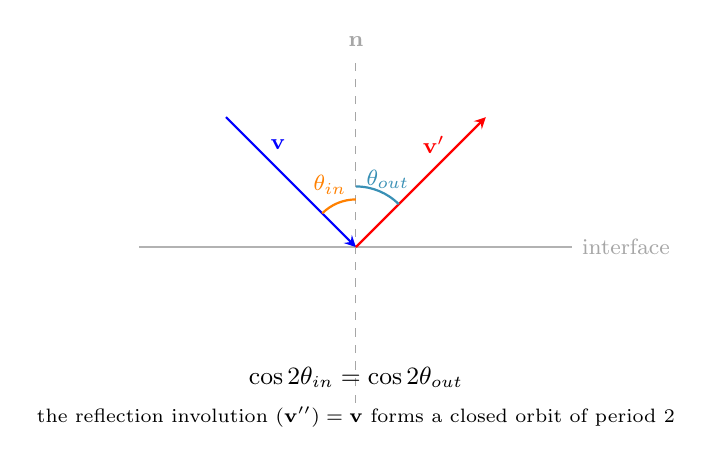
\begin{tikzpicture}[scale=1.1,>=stealth]

        \draw[gray!60, thick] (-2.5,0) -- (2.5,0);
        \node[gray!70, font=\footnotesize, right] at (2.5,0) {interface};

        \draw[gray!70, dashed] (0,-1.8) -- (0,2.2);
        \node[gray!70, font=\footnotesize, above] at (0,2.2) {$\mathbf{n}$};

        \draw[->, thick, blue] (-1.5,1.5) -- (0,0);
        \node[blue, font=\footnotesize] at (-0.9, 1.18) {$\mathbf{v}$};

        \draw[->, thick, red] (0,0) -- (1.5,1.5);
        \node[red, font=\footnotesize] at (0.9, 1.18) {$\mathbf{v}'$};

        \draw[orange, thick] (0,0) ++(90:0.55) arc (90:135:0.55);
        \node[orange, font=\footnotesize] at (-0.30, 0.72) {$\theta_{\text{in}}$};

        \draw[cyan!70!black, thick] (0,0) ++(90:0.7) arc (90:45:0.7);
        \node[cyan!70!black, font=\footnotesize] at (0.37, 0.78) {$\theta_{\text{out}}$};

        \node[font=\small\bfseries, below=1.4cm] at (0,0)
            {$\cos 2\theta_{\text{in}}=\cos 2\theta_{\text{out}}$};
        \node[font=\scriptsize, align=center, below=1.9cm] at (0,0)
            {the reflection involution $(\mathbf{v}'')=\mathbf{v}$ forms a closed orbit of period $2$};
    \end{tikzpicture}
    \caption{Conservation of the double-angle cosine similarity under reflection. The double-angle cosine $\cos 2\theta_{\text{in}}$ of the incident direction $\mathbf{v}$ with the normal $\mathbf{n}$ is unchanged after reflection. Reflection is an involution: two reflections return to $\mathbf{v}$, constituting the smallest periodic structure of this chapter (Definition \ref{def:reflection_vector}).}
    \label{fig:reflection_conservation}
\end{figure}

\begin{proof}
Compute the square of the modulus:
\[\|\mathbf{v}'\|^2 = \|\mathbf{v} - 2(\mathbf{v}\cdot\mathbf{n})\mathbf{n}\|^2 = \|\mathbf{v}\|^2 - 4(\mathbf{v}\cdot\mathbf{n})^2 + 4(\mathbf{v}\cdot\mathbf{n})^2\|\mathbf{n}\|^2 = \|\mathbf{v}\|^2,\]
because $\|\mathbf{n}\|=1$. Reflect twice: $\mathbf{v}'' = \mathbf{v}' - 2(\mathbf{v}'\cdot\mathbf{n})\mathbf{n} = \mathbf{v} - 2(\mathbf{v}\cdot\mathbf{n})\mathbf{n} - 2((\mathbf{v} - 2(\mathbf{v}\cdot\mathbf{n})\mathbf{n})\cdot\mathbf{n})\mathbf{n}$. Compute the inner product: $(\mathbf{v} - 2(\mathbf{v}\cdot\mathbf{n})\mathbf{n})\cdot\mathbf{n} = \mathbf{v}\cdot\mathbf{n} - 2(\mathbf{v}\cdot\mathbf{n}) = -\mathbf{v}\cdot\mathbf{n}$. Substituting gives $\mathbf{v}'' = \mathbf{v} - 2(\mathbf{v}\cdot\mathbf{n})\mathbf{n} - 2(-\mathbf{v}\cdot\mathbf{n})\mathbf{n} = \mathbf{v}$. Hence reflection is an involution. The double-angle cosine similarity is unchanged because the angle of reflection equals the angle of incidence: $\theta_{\text{out}} = \theta_{\text{in}}$, hence $\cos 2\theta_{\text{out}} = \cos 2\theta_{\text{in}}$.
\end{proof}

\begin{definition}[Refraction---the scaling of the sine tendency]\label{def:refraction_vector}
Let the incident vector be $\mathbf{v}$, let the normal be $\mathbf{n}$ (a unit vector), and let the angle of incidence be $\theta_1$. The refracted vector $\mathbf{v}''$ lies in the plane spanned by $\mathbf{v}$ and $\mathbf{n}$, and its angle $\theta_2$ with the normal satisfies Snell's law:
\[n_1 \sin\theta_1 = n_2 \sin\theta_2.\]
Refraction embodies the modulation of the rotation direction ($i$-symmetry) by multiplicative scaling reflection symmetry ($c \neq 1$): the refractive indices $n_1, n_2$ act as proportionality factors scaling the sine tendencies in the two media. The modulus of the refracted vector is determined by the conservation of energy or by the amplitude coefficients, and its direction is uniquely determined by Snell's law (within the plane of incidence).
\end{definition}

\begin{figure}[htbp]
    \centering
    \begin{tikzpicture}[scale=1.1,>=stealth]

        \draw[gray!60, thick] (-3.2,0) -- (3.2,0);
        \node[gray!70, font=\footnotesize, right] at (3.2,0) {interface};

        \draw[gray!70, dashed] (0,-2.0) -- (0,2.2);
        \node[gray!70, font=\footnotesize, above] at (0,2.2) {$\mathbf{n}$};

        \draw[->, thick, blue] (-2.4,1.7) -- (0,0);
        \node[blue, font=\footnotesize] at (-1.6,0.75) {$\mathbf{v}$};
        \draw[orange] (0,0.8) arc (90:126:0.8);
        \node[orange, font=\footnotesize] at (-0.45,1.05) {$\theta_1$};
        \node[blue, font=\footnotesize] at (-2.3,1.95) {$n_1$};

        \draw[->, thick, red] (0,0) -- (1.8,-1.7);
        \node[red, font=\footnotesize] at (1.4,-0.8) {$\mathbf{v}''$};
        \draw[orange] (0,-0.8) arc (-90:-42:0.8);
        \node[orange, font=\footnotesize] at (0.45,-1.05) {$\theta_2$};
        \node[red, font=\footnotesize] at (2.3,-1.95) {$n_2$};

        \node[font=\small\bfseries, below=2.5cm] at (0,0)
            {$n_1\sin\theta_1 = n_2\sin\theta_2$};
        \node[font=\scriptsize, align=center, below=3.0cm] at (0,0)
            {the sine tendency is conserved along the interface normal; the refractive indices $n_1,n_2$ are scaling factors};
    \end{tikzpicture}
    \caption{Snell's law of refraction and the scaling of the sine tendency. The sine tendency $n\sin\theta$ of the incident and refracted directions is conserved at the interface, and the refractive indices $n_1,n_2$ act as scaling factors modulating the rotation direction. When $n_1\sin\theta_1 > n_2$ total internal reflection occurs (Proposition \ref{prop:critical_angle}).}
    \label{fig:refraction_snell}
\end{figure}

\begin{proposition}[The critical angle of refraction]\label{prop:critical_angle}
When $n_1 > n_2$ and the angle of incidence $\theta_1$ exceeds the critical angle $\theta_c = \arcsin(n_2/n_1)$, we have $\sin\theta_1 > n_2/n_1$, and Snell's law requires $\sin\theta_2 > 1$, which has no solution in the real domain; refraction no longer occurs, and the light is entirely reflected back into the original medium (total internal reflection).
\end{proposition}

\begin{proof}
By Snell's law, $\sin\theta_2 = \frac{n_1}{n_2}\sin\theta_1$. If $\sin\theta_1 > \frac{n_2}{n_1}$, then $\sin\theta_2 > 1$, but the range of the sine function is $[-1,1]$, so there is no real solution. The critical angle is defined as $\theta_c = \arcsin(n_2/n_1)$.
\end{proof}

\section{Directional composition in complex and quaternion multiplication, and exponential similarity}
\label{sec:complex_quaternion_exponential_similarity}

This section treats complex numbers and quaternions according to the unified logic of `angle difference / angle sum': the difference-angle operator and the sum-angle operator encode `rotation difference' and `rotational composition' respectively, their real parts corresponding to the cosine family and their imaginary parts (or vector parts) to the sine family. In the complex case left multiplication is a rotation; in the quaternion case the conjugation action gives a three-dimensional rotation. When the axes coincide, the quaternion case degenerates strictly to the angle difference and angle sum of the complex case.

\subsection{Complex multiplication: sum-angle tendency and rotational composition}

\begin{proposition}[Complex multiplication---sum-angle tendency and rotational composition]\label{prop:complex_multiplication}
Regard the complex number $z=a+bi$ as a vector in $\mathbb R^2$. Let
\[
z_1=r_1e^{i\alpha},\qquad z_2=r_2e^{i\beta}.
\]
Then the real and imaginary parts of the product $z_1z_2$ correspond respectively to the \textbf{basic sum-angle cosine tendency} and the \textbf{basic sum-angle sine tendency}:
\[
z_1z_2
=
\operatorname{cosine\_tendency}_+(\mathbf a,\mathbf b)
+
i\operatorname{sine\_tendency}_+(\mathbf a,\mathbf b),
\]
where $\mathbf a,\mathbf b$ correspond to $z_1,z_2$ respectively. Complex multiplication adds the two rotation angles and multiplies the two moduli: the addition of arguments corresponds to directional composition along the rotation direction, and the multiplication of moduli corresponds to scale composition along the proportional direction.
\end{proposition}

\begin{proof}
By complex multiplication,
\[
z_1z_2
=
r_1r_2e^{i(\alpha+\beta)}
=
r_1r_2\bigl[\cos(\alpha+\beta)+i\sin(\alpha+\beta)\bigr].
\]
Since $r_1r_2=\|\mathbf a\|\|\mathbf b\|$, the real part is
\[
\|\mathbf a\|\|\mathbf b\|\cos(\alpha+\beta)
=
\operatorname{cosine\_tendency}_+(\mathbf a,\mathbf b),
\]
and the imaginary part is
\[
\|\mathbf a\|\|\mathbf b\|\sin(\alpha+\beta)
=
\operatorname{sine\_tendency}_+(\mathbf a,\mathbf b).
\]
This completes the proof.
\end{proof}

\begin{remark}
Complex multiplication corresponds to the `sum angle', that is, the two directions are each independent and are then composed into a new direction. What it describes is the composition of rotations, not the relative difference between two directions. The relative difference is described by the complex exponential similarity below.
\end{remark}

\begin{definition}[Complex exponential difference-angle and sum-angle operators]\label{def:complex_diff_sum}
Let $z_1=r_1e^{i\alpha}$ and $z_2=r_2e^{i\beta}$, both non-zero. Define
\[
\boxed{
D_{\mathbb C}(z_1,z_2):=\frac{z_1\overline{z_2}}{|z_1|\,|z_2|}
}
\]
to be the \textbf{complex exponential difference-angle operator} (angle-difference operator) of $z_1$ and $z_2$;
\[
\boxed{
S_{\mathbb C}(z_1,z_2):=\frac{z_1z_2}{|z_1|\,|z_2|}
}
\]
to be the \textbf{complex exponential sum-angle operator} (angle-sum operator) of $z_1$ and $z_2$. Both are unit complex numbers, and they can be written as
\[
D_{\mathbb C}(z_1,z_2)=e^{i(\alpha-\beta)},\qquad
S_{\mathbb C}(z_1,z_2)=e^{i(\alpha+\beta)}.
\]
\end{definition}

\begin{proposition}[The complex exponential difference-angle operator is a two-dimensional rotation-difference operator]\label{prop:complex_exp_similarity_rotation_operator}
Let $z_1,z_2\in\mathbb C^\times$. Then $D_{\mathbb C}(z_1,z_2)$ gives, through multiplication, the two-dimensional rotation from the unit direction of $z_2$ to the unit direction of $z_1$:
\[
\boxed{
D_{\mathbb C}(z_1,z_2)\cdot \frac{z_2}{|z_2|}
=
\frac{z_1}{|z_1|}
}
\]
that is, $D_{\mathbb C}(z_1,z_2)$ is a two-dimensional rotation-difference operator. Its argument is $\alpha-\beta$, its real part corresponds to the basic difference-angle cosine similarity and its imaginary part to the basic difference-angle sine similarity; in parallel, the argument of $S_{\mathbb C}(z_1,z_2)$ is $\alpha+\beta$, and its real and imaginary parts correspond respectively to the basic sum-angle cosine tendency and the basic sum-angle sine tendency.
\end{proposition}

\begin{proof}
By the definition and $z_2\overline{z_2}=|z_2|^2$,
\[
D_{\mathbb C}(z_1,z_2)\cdot\frac{z_2}{|z_2|}
=
\frac{z_1\overline{z_2}}{|z_1|\,|z_2|}\cdot\frac{z_2}{|z_2|}
=
\frac{z_1\,|z_2|^2}{|z_1|\,|z_2|^2}
=
\frac{z_1}{|z_1|}.
\]
Hence $D_{\mathbb C}(z_1,z_2)$ sends the unit direction of $z_2$ to the unit direction of $z_1$, acting by complex multiplication (that is, a two-dimensional rotation), and no conjugation is needed. From
\[
D_{\mathbb C}(z_1,z_2)=e^{i(\alpha-\beta)}=\cos(\alpha-\beta)+i\sin(\alpha-\beta)
\]
the correspondence of the argument with the real and imaginary parts is obtained directly; the correspondence on the $S_{\mathbb C}$ side has already been given by Proposition \ref{prop:complex_multiplication}. This completes the proof.
\end{proof}

\begin{figure}[htbp]
    \centering
    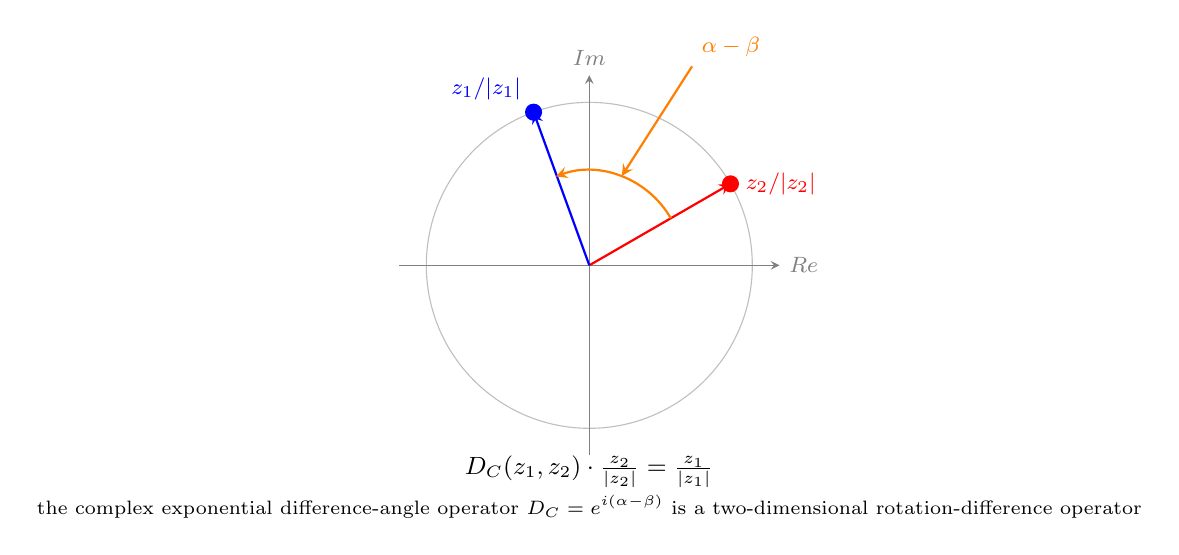
\begin{tikzpicture}[scale=1.15,>=stealth]

        \draw[gray!50] (0,0) circle (1.8);
        \draw[->, gray] (-2.1,0) -- (2.1,0) node[right, font=\footnotesize] {$\operatorname{Re}$};
        \draw[->, gray] (0,-2.1) -- (0,2.1) node[above, font=\footnotesize] {$\operatorname{Im}$};

        \filldraw[red] (30:1.8) circle (2.5pt);
        \node[red, font=\footnotesize, right=2pt] at (30:1.8) {$z_2/|z_2|$};
        \draw[->, thick, red] (0,0) -- (30:1.8);

        \filldraw[blue] (110:1.8) circle (2.5pt);
        \node[blue, font=\footnotesize, above left=1pt] at (110:1.8) {$z_1/|z_1|$};
        \draw[->, thick, blue] (0,0) -- (110:1.8);

        \draw[->, thick, orange] (0.9,0.52) arc (30:110:1.05);
        \node[orange, font=\footnotesize] (anglelabel) at (1.564, 2.414) {$\alpha-\beta$};
        \draw[->, thick, orange] (anglelabel.south west) -- (70:1.05);

        \node[font=\small\bfseries, below=2.3cm] at (0,0)
            {$D_{\mathbb{C}}(z_1,z_2)\cdot\frac{z_2}{|z_2|}=\frac{z_1}{|z_1|}$};
        \node[font=\scriptsize, align=center, below=2.8cm] at (0,0)
            {the complex exponential difference-angle operator $D_{\mathbb{C}}=e^{i(\alpha-\beta)}$ is a two-dimensional rotation-difference operator};
    \end{tikzpicture}
    \caption{The rotation-difference action of the complex exponential difference-angle operator. $D_{\mathbb{C}}(z_1,z_2)=e^{i(\alpha-\beta)}$ rotates the unit direction of $z_2$ exactly onto the unit direction of $z_1$, realising the `rotation difference from $z_2$ to $z_1$' (Proposition \ref{prop:complex_exp_similarity_rotation_operator}).}
    \label{fig:complex_exp_rotation_operator}
\end{figure}

\begin{remark}[The composition law of the complex exponential difference-angle operator]\label{rem:complex_exp_similarity_composition}
Let $z_1,z_2,z_3\in\mathbb C^\times$. From the definition one obtains directly
\[
D_{\mathbb C}(z_1,z_2)\,D_{\mathbb C}(z_2,z_3)=D_{\mathbb C}(z_1,z_3),
\]
that is, the complex exponential difference-angle operator satisfies the composition law of rotation differences. This composition law is completely parallel to \cref{prop:quaternion_exp_similarity_composition} in the quaternion case; the difference between the two lies in the fact that complex multiplication is commutative whilst quaternion multiplication is not (see \cref{rem:quaternion_exp_similarity_noncommutative}), which is precisely the structural difference between two-dimensional and three-dimensional rotation differences.
\end{remark}

\subsection{Quaternion multiplication: non-commutative rotational composition}

\begin{proposition}[Quaternion multiplication---non-commutative rotational direction]\label{prop:quaternion_multiplication}
Quaternion multiplication is the non-commutative generalisation of complex multiplication, realising three-dimensional rotational direction. A unit quaternion $q=e^{\mathbf u\theta}$ acts on a pure imaginary vector $v$ through conjugation
\[
v\longmapsto qvq^{-1}
\]
producing the effect of a rotation by $2\theta$ about the axis $\mathbf u$. The product of two unit quaternions
\[
q_1q_2=e^{\mathbf u_1\theta_1}e^{\mathbf u_2\theta_2}
\]
corresponds to the composition of two three-dimensional rotations; since in general $q_1q_2\neq q_2q_1$, the result of the composition depends on the order. This is the generalisation of the rotation direction from the commutative group $U(1)$ to the non-commutative group $SU(2)$.
\end{proposition}

\begin{proof}
Write the unit quaternion as
\[
q=\cos\theta+\mathbf u\sin\theta,
\]
where $\mathbf u$ is a unit pure imaginary quaternion with $\mathbf u^2=-1$, and
\[
q^{-1}=\cos\theta-\mathbf u\sin\theta.
\]
For a pure imaginary quaternion $v$, the image of the conjugation action is still a pure imaginary quaternion:
\[
\overline{qvq^{-1}}
=
\overline{q^{-1}}\,\bar v\,\bar q
=
q\,(-v)\,q^{-1}
=
-qvq^{-1}.
\]
Decompose $v$ along the axis as
\[
v=v_\parallel+v_\perp,
\]
where $v_\parallel\parallel \mathbf u$ and $v_\perp\perp \mathbf u$. The parallel component satisfies $\mathbf u v_\parallel=v_\parallel \mathbf u$, hence
\[
qv_\parallel q^{-1}=v_\parallel.
\]
For the perpendicular component, since $\mathbf u\cdot v_\perp=0$, the multiplication of pure imaginary quaternions satisfies
\[
\mathbf u v_\perp=\mathbf u\times v_\perp,\qquad
v_\perp \mathbf u=-\mathbf u\times v_\perp.
\]
Therefore
\begin{align*}
qv_\perp q^{-1}
&=
(\cos\theta+\mathbf u\sin\theta)\,v_\perp\,(\cos\theta-\mathbf u\sin\theta) \\
&=
\cos^2\theta\,v_\perp
-\cos\theta\sin\theta\,(v_\perp \mathbf u)
+\sin\theta\cos\theta\,(\mathbf u v_\perp)
-\sin^2\theta\,(\mathbf u v_\perp \mathbf u).
\end{align*}
Using $v_\perp \mathbf u=-\mathbf u v_\perp$ and the triple cross-product identity
\[
(\mathbf u\times v_\perp)\times \mathbf u=v_\perp
\]
(since $\mathbf u\perp v_\perp$ and $\|\mathbf u\|=1$), we obtain
\[
qv_\perp q^{-1}
=
(\cos^2\theta-\sin^2\theta)\,v_\perp
+
2\sin\theta\cos\theta\,(\mathbf u\times v_\perp)
=
\cos 2\theta\,v_\perp
+
\sin 2\theta\,(\mathbf u\times v_\perp).
\]
This is precisely the Rodrigues formula for a rotation by angle $2\theta$ about the axis $\mathbf u$. Hence the conjugation action $v\mapsto qvq^{-1}$ is a rotation by $2\theta$ about the axis $\mathbf u$.

The conjugation action corresponding to the product of two unit quaternions is
\[
v\longmapsto (q_1q_2)v(q_1q_2)^{-1}
=
q_1\,(q_2 v q_2^{-1})\,q_1^{-1},
\]
that is, the composite of first a rotation by $2\theta_2$ about $\mathbf u_2$ and then a rotation by $2\theta_1$ about $\mathbf u_1$. Since in general $q_1q_2\neq q_2q_1$, the order of composition of three-dimensional rotations is not commutative, and this is precisely the source of the non-commutativity of $SO(3)$; under this conjugation correspondence the unit quaternions form the double cover $SU(2)$ of $SO(3)$. This completes the proof.
\end{proof}

\subsection{Difference-angle and sum-angle quaternions}

\begin{definition}[The polar form and angle of a quaternion]\label{def:quaternion_polar}
Let $q\in\mathbb H^\times$, with $q$ not a negative real number. Then $q$ can be written uniquely in \textbf{polar form}
\[
q=|q|\Bigl(\cos\theta+\mathbf u\sin\theta\Bigr),
\]
where $\theta\in[0,\pi)$ is called the \textbf{argument} (or \textbf{angle}) of $q$, and $\mathbf u$ is a unit pure imaginary quaternion ($\mathbf u^2=-1$), called the \textbf{axis} of $q$. When $q$ is a negative real number, we adopt the convention $\theta=\pi$, with $\mathbf u$ an arbitrary unit pure imaginary quaternion.
\end{definition}

\begin{definition}[Difference-angle and sum-angle quaternions]\label{def:quaternion_diff_sum}
Let $p,q\in\mathbb H^\times$. Define
\[
\boxed{
D_{\mathbb H}(p,q):=\frac{p\overline q}{|p|\,|q|}
}
\]
to be the \textbf{difference-angle quaternion} (angle-difference operator) of $p$ and $q$;
\[
\boxed{
S_{\mathbb H}(p,q):=\frac{pq}{|p|\,|q|}
}
\]
to be the \textbf{sum-angle quaternion} (angle-sum operator) of $p$ and $q$. Both are unit quaternions.
\end{definition}

\begin{lemma}[The scalar-vector decomposition of the difference-angle and sum-angle quaternions]\label{lem:quaternion_diff_sum_decomposition}
Let $p=|p|e^{\mathbf u\alpha}$, $q=|q|e^{\mathbf v\beta}$, that is,
\[
p=|p|\bigl(\cos\alpha+\mathbf u\sin\alpha\bigr),\qquad
q=|q|\bigl(\cos\beta+\mathbf v\sin\beta\bigr).
\]
Then the difference-angle quaternion expands as
\[
\begin{aligned}
D_{\mathbb H}(p,q)
={}& \underbrace{\bigl(\cos\alpha\cos\beta+\sin\alpha\sin\beta\,(\mathbf u\cdot\mathbf v)\bigr)}_{\text{scalar part}} \\
&+ \underbrace{\bigl(\sin\alpha\cos\beta\,\mathbf u-\cos\alpha\sin\beta\,\mathbf v
   -\sin\alpha\sin\beta\,(\mathbf u\times\mathbf v)\bigr)}_{\text{vector part}},
\end{aligned}
\]
and the sum-angle quaternion expands as
\[
\begin{aligned}
S_{\mathbb H}(p,q)
={}& \underbrace{\bigl(\cos\alpha\cos\beta-\sin\alpha\sin\beta\,(\mathbf u\cdot\mathbf v)\bigr)}_{\text{scalar part}} \\
&+ \underbrace{\bigl(\sin\alpha\cos\beta\,\mathbf u+\cos\alpha\sin\beta\,\mathbf v
   +\sin\alpha\sin\beta\,(\mathbf u\times\mathbf v)\bigr)}_{\text{vector part}}.
\end{aligned}
\]
When $\mathbf u=\mathbf v$ the cross terms vanish, and the two degenerate respectively to
\[
D_{\mathbb H}(p,q)=\cos(\alpha-\beta)+\mathbf u\sin(\alpha-\beta),\qquad
S_{\mathbb H}(p,q)=\cos(\alpha+\beta)+\mathbf u\sin(\alpha+\beta),
\]
completely parallel to the complex case: the angle of the difference-angle quaternion is $\alpha-\beta$, the angle of the sum-angle quaternion is $\alpha+\beta$, and both axes are $\mathbf u$.
\end{lemma}

\begin{proof}
Use the multiplication formula for pure imaginary quaternions
\[
\mathbf u\mathbf v=-\mathbf u\cdot\mathbf v+\mathbf u\times\mathbf v,
\]
together with $e^{\mathbf u\alpha}=\cos\alpha+\mathbf u\sin\alpha$, $e^{-\mathbf v\beta}=\cos\beta-\mathbf v\sin\beta$ and $e^{\mathbf v\beta}=\cos\beta+\mathbf v\sin\beta$.

First expand the difference-angle quaternion:
\[
D_{\mathbb H}(p,q)=e^{\mathbf u\alpha}e^{-\mathbf v\beta}
=
(\cos\alpha+\mathbf u\sin\alpha)(\cos\beta-\mathbf v\sin\beta).
\]
The scalar part is
\[
\cos\alpha\cos\beta-(\mathbf u\cdot(-\mathbf v))\sin\alpha\sin\beta
=
\cos\alpha\cos\beta+\sin\alpha\sin\beta\,(\mathbf u\cdot\mathbf v),
\]
and the vector part is
\[
\sin\alpha\cos\beta\,\mathbf u-\cos\alpha\sin\beta\,\mathbf v
+\sin\alpha\sin\beta\,(\mathbf u\times(-\mathbf v)),
\]
where $\mathbf u\times(-\mathbf v)=-\mathbf u\times\mathbf v$, so the vector part is
\[
\sin\alpha\cos\beta\,\mathbf u-\cos\alpha\sin\beta\,\mathbf v-\sin\alpha\sin\beta\,(\mathbf u\times\mathbf v).
\]
Likewise expand the sum-angle quaternion:
\[
S_{\mathbb H}(p,q)=e^{\mathbf u\alpha}e^{\mathbf v\beta}
=
(\cos\alpha+\mathbf u\sin\alpha)(\cos\beta+\mathbf v\sin\beta).
\]
The scalar part is
\[
\cos\alpha\cos\beta-(\mathbf u\cdot\mathbf v)\sin\alpha\sin\beta,
\]
and the vector part is
\[
\sin\alpha\cos\beta\,\mathbf u+\cos\alpha\sin\beta\,\mathbf v+\sin\alpha\sin\beta\,(\mathbf u\times\mathbf v).
\]
When $\mathbf u=\mathbf v$, $\mathbf u\cdot\mathbf v=1$ and $\mathbf u\times\mathbf v=0$; substituting gives the degenerate formulae. This completes the proof.
\end{proof}

\begin{proposition}[The difference-angle quaternion is a three-dimensional rotation-difference operator]\label{prop:quaternion_exp_similarity_rotation_operator}
Let $p,q\in\mathbb H^\times$. Then $D_{\mathbb H}(p,q)$ gives, through the conjugation action, the three-dimensional rotation from the unit direction of $q$ to the unit direction of $p$:
\[
\boxed{
D_{\mathbb H}(p,q)\cdot \frac{q}{|q|}\cdot D_{\mathbb H}(p,q)^{-1}
=
\frac{p}{|p|}
}
\]
that is, $D_{\mathbb H}(p,q)$ is a rotation-difference operator. Its scalar part corresponds to the quaternion cosine similarity and the modulus of its vector part to the quaternion sine similarity.
\end{proposition}

\begin{figure}[htbp]
    \centering
    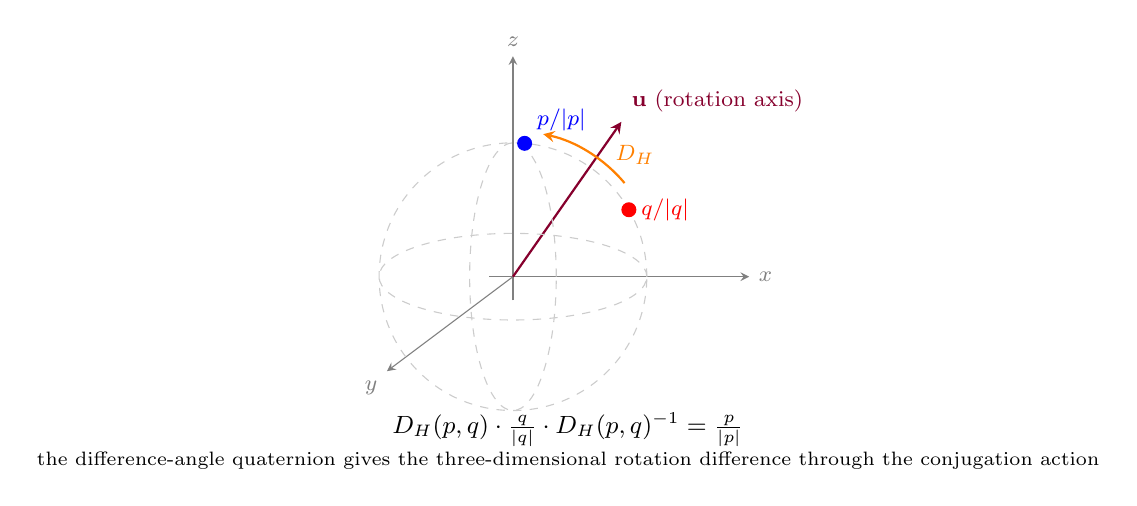
\begin{tikzpicture}[scale=1.0,>=stealth]

        \draw[->, gray] (-0.3,0) -- (3.0,0) node[right, font=\footnotesize] {$x$};
        \draw[->, gray] (0,-0.3) -- (0,2.8) node[above, font=\footnotesize] {$z$};
        \draw[->, gray] (0,0) -- (-1.6,-1.2) node[below left, font=\footnotesize] {$y$};

        \draw[->, thick, purple!70!black] (0,0) -- (55:2.4)
            node[above right, font=\footnotesize] {$\mathbf{u}$ (rotation axis)};

        \draw[gray!40, dashed] (0,0) circle (1.7);
        \draw[gray!40, dashed] (0,0) ellipse (1.7 and 0.55);
        \draw[gray!40, dashed] (0,0) ellipse (0.55 and 1.7);

        \coordinate (P) at (30:1.7);
        \filldraw[red] (P) circle (2.5pt);
        \node[red, font=\footnotesize, right=1pt] at (P) {$q/|q|$};

        \coordinate (Q) at (85:1.7);
        \filldraw[blue] (Q) circle (2.5pt);
        \node[blue, font=\footnotesize, above right=1pt] at (Q) {$p/|p|$};

        \draw[->, thick, orange] (40:1.85) arc (40:78:1.85);
        \node[orange, font=\footnotesize] at (1.55,1.55) {$D_{\mathbb{H}}$};

        \node[font=\small\bfseries, below=1.4cm] at (0.7,-0.2)
            {$D_{\mathbb{H}}(p,q)\cdot\frac{q}{|q|}\cdot D_{\mathbb{H}}(p,q)^{-1}=\frac{p}{|p|}$};
        \node[font=\scriptsize, align=center, below=1.9cm] at (0.7,-0.2)
            {the difference-angle quaternion gives the three-dimensional rotation difference through the conjugation action};
    \end{tikzpicture}
    \caption{The three-dimensional rotation-difference action of the difference-angle quaternion. $D_{\mathbb{H}}(p,q)=p\overline{q}/(|p||q|)$ sends the unit direction of $q$ to the unit direction of $p$ through the conjugation action $v\mapsto DvD^{-1}$, realising a three-dimensional rotation-difference operator. When the axes coincide it degenerates to the angle difference of the complex case (Proposition \ref{prop:quaternion_exp_similarity_rotation_operator}, Theorem \ref{thm:quaternion_sum_rotation_degeneration}).}
    \label{fig:quaternion_conjugation_rotation}
\end{figure}

\begin{proof}
By the definition
\[
D_{\mathbb H}(p,q)=\frac{p\overline q}{|p||q|},
\]
hence
\[
D_{\mathbb H}(p,q)\cdot \frac{q}{|q|}\cdot D_{\mathbb H}(p,q)^{-1}
=
\frac{p\overline q}{|p||q|}\cdot\frac{q}{|q|}\cdot\frac{q\overline p}{|q||p|}.
\]
Using $q\overline q=|q|^2$ and $\overline q\,q=|q|^2$, we obtain
\[
D_{\mathbb H}(p,q)\cdot \frac{q}{|q|}\cdot D_{\mathbb H}(p,q)^{-1}
=
\frac{p\,|q|^2\,\overline p}{|p|^2|q|^2|q|}
=
\frac{p\,\overline p}{|p|^2}\cdot\frac{q}{|q|}.
\]
When $p,q$ are unit quaternions, $p\overline p=|p|^2=1$ and $|q|=1$, and the above expression becomes
\[
D_{\mathbb H}(p,q)\,q\,D_{\mathbb H}(p,q)^{-1}=p.
\]
The general case is reduced to this by normalisation. Hence $D_{\mathbb H}(p,q)$ sends the unit direction of $q$ to the unit direction of $p$ through the conjugation action. The decomposition into scalar and vector parts is given by Lemma \ref{lem:quaternion_diff_sum_decomposition}. This completes the proof.
\end{proof}

\begin{proposition}[The composition law of the difference-angle quaternion]\label{prop:quaternion_exp_similarity_composition}
Let $p,q,r\in\mathbb H^\times$. Then
\[
D_{\mathbb H}(p,q)\,D_{\mathbb H}(q,r)
=
D_{\mathbb H}(p,r).
\]
That is, the difference-angle quaternion satisfies the composition law of rotation differences.
\end{proposition}

\begin{proof}
By the definition,
\[
D_{\mathbb H}(p,q)D_{\mathbb H}(q,r)
=
\frac{p\overline q}{|p||q|}\cdot\frac{q\overline r}{|q||r|}
=
\frac{p|q|^2\overline r}{|p||q|^2|r|}
=
\frac{p\overline r}{|p||r|}
=
D_{\mathbb H}(p,r).
\]
This completes the proof.
\end{proof}

\begin{theorem}[The sum-angle quaternion is a three-dimensional rotational composition operator]\label{thm:quaternion_sum_rotation_operator}
Let $p,q\in\mathbb H^\times$. Then $S_{\mathbb H}(p,q)=pq/(|p||q|)$ gives, through the conjugation action, a rotational composition: first $q$ gives a rotation, then $p$ gives a rotation, and the composite result is the conjugation action of $S_{\mathbb H}(p,q)$.
\end{theorem}

\begin{proof}
For a pure imaginary quaternion $v$, the conjugation action satisfies
\[
(pq)v(pq)^{-1}=p\bigl(qvq^{-1}\bigr)p^{-1}.
\]
Hence acting first by $q$ and then by $p$ is equivalent to acting by $pq$. After normalisation, this gives that $S_{\mathbb H}(p,q)=pq/(|p||q|)$ yields a rotational composition through the conjugation action. This completes the proof.
\end{proof}

\begin{theorem}[The degeneracy of the sum-angle quaternion when the axes coincide is parallel to the complex case]\label{thm:quaternion_sum_rotation_degeneration}
When $p,q$ have the same axis ($\mathbf u=\mathbf v$), the difference-angle quaternion and the sum-angle quaternion degenerate respectively to
\[
D_{\mathbb H}(p,q)=e^{\mathbf u(\alpha-\beta)},\qquad
S_{\mathbb H}(p,q)=e^{\mathbf u(\alpha+\beta)},
\]
completely parallel to the complex exponential similarity and the complex exponential tendency. The scalar part corresponds to the cosine family, and the modulus of the vector part to the sine family.
\end{theorem}

\begin{proof}
By Lemma \ref{lem:quaternion_diff_sum_decomposition}, when the axes coincide the difference-angle quaternion becomes
\[
D_{\mathbb H}(p,q)=\cos(\alpha-\beta)+\mathbf u\sin(\alpha-\beta)=e^{\mathbf u(\alpha-\beta)},
\]
and the sum-angle quaternion becomes
\[
S_{\mathbb H}(p,q)=\cos(\alpha+\beta)+\mathbf u\sin(\alpha+\beta)=e^{\mathbf u(\alpha+\beta)}.
\]
The scalar parts are $\cos(\alpha-\beta)$ and $\cos(\alpha+\beta)$ respectively, corresponding to the cosine similarity and the cosine tendency; the moduli of the vector parts are $|\sin(\alpha-\beta)|$ and $|\sin(\alpha+\beta)|$ respectively, corresponding to the sine similarity and the sine tendency. In the complex case there is only one fixed axis $i$, so the above degeneracy is precisely the complex exponential similarity and the complex exponential tendency. This completes the proof.
\end{proof}

\begin{theorem}[The inner-product and cross-product decomposition of the quaternion exponential tendency]\label{thm:quaternion_exp_tendency_geometry}
Let $p,q\in\mathbb H^\times$. Write
\[
p=p_0+\mathbf p,\qquad q=q_0+\mathbf q,
\]
where $p_0,q_0\in\mathbb R$ and $\mathbf p,\mathbf q$ are pure imaginary quaternions. Then
\[
\operatorname{Tendency}^{\mathbb H}(p,q):=p\overline q
\]
satisfies
\[
\operatorname{Sc}\bigl(\operatorname{Tendency}^{\mathbb H}(p,q)\bigr)
=
p_0q_0+\mathbf p\cdot\mathbf q
=
\langle p,q\rangle,
\]
that is, the scalar part is the quaternion inner product, which is also the quaternion cosine tendency. If $p,q$ are pure imaginary quaternions, that is, $p=\mathbf p$, $q=\mathbf q$, then
\[
\operatorname{Vec}\bigl(\operatorname{Tendency}^{\mathbb H}(p,q)\bigr)
=
-\mathbf p\times\mathbf q,
\]
and hence
\[
\left\|\operatorname{Vec}\bigl(\operatorname{Tendency}^{\mathbb H}(p,q)\bigr)\right\|
=
\|\mathbf p\|\,\|\mathbf q\|\sin\theta,
\]
that is, the modulus of the vector part is the quaternion sine tendency, whose direction is given by the cross product.
\end{theorem}

\begin{proof}
By the quaternion multiplication formula
\[
(a+\mathbf A)(b+\mathbf B)
=
ab-\mathbf A\cdot\mathbf B
+
a\mathbf B+b\mathbf A+\mathbf A\times\mathbf B.
\]
Take $b=q_0$ and $\mathbf B=-\mathbf q$; then
\[
p\overline q=(p_0+\mathbf p)(q_0-\mathbf q).
\]
The scalar part is
\[
p_0q_0-\mathbf p\cdot(-\mathbf q)=p_0q_0+\mathbf p\cdot\mathbf q.
\]
If $p_0=q_0=0$, then
\[
p\overline q=\mathbf p(-\mathbf q)=-\mathbf p\times\mathbf q+\mathbf p\cdot\mathbf q,
\]
where the scalar part is $\mathbf p\cdot\mathbf q$ and the vector part is $-\mathbf p\times\mathbf q$. Hence the modulus of the vector part is
\[
\|\mathbf p\times\mathbf q\|=\|\mathbf p\|\,\|\mathbf q\|\sin\theta.
\]
This completes the proof.
\end{proof}

\begin{example}[A numerical example of the quaternion exponential similarity]\label{ex:quaternion_exp_similarity_example}
Take
\[
p=i,\qquad q=1.
\]
Then
\[
D_{\mathbb H}(p,q)=\frac{i\cdot 1}{1\cdot 1}=i.
\]
Write
\[
i=\cos\frac{\pi}{2}+i\sin\frac{\pi}{2},
\]
so the scalar part is $\cos(\pi/2)=0$, the vector part is $i\sin(\pi/2)=i$, and the modulus is $1$. Through the conjugation action it gives the three-dimensional rotation difference from $1$ to $i$: a rotation by angle $\pi$ about the $i$ axis. Its difference-angle quaternion and sum-angle quaternion (here $q=1$, so the two are equal) are both $i$, embodying the consistency of the quaternion case with the complex case whilst retaining the information of the three-dimensional rotation axis.
\end{example}

\begin{remark}[The non-commutativity of the quaternion difference-angle quaternion]\label{rem:quaternion_exp_similarity_noncommutative}
The complex exponential similarity is unchanged under simultaneous left multiplication or simultaneous right multiplication by a common factor; the quaternion difference-angle quaternion is different: right multiplication by a common factor leaves it unchanged, whilst left multiplication by a common factor in general gives a conjugation transformation
\[
D_{\mathbb H}(rp,rq)=r\,D_{\mathbb H}(p,q)\,\overline r.
\]
This is precisely the manifestation of quaternion non-commutativity at the level of similarity. If $r$ commutes with $D_{\mathbb H}(p,q)$, the conjugation transformation degenerates to invariance. The quaternion difference-angle quaternion therefore records not only the `rotation angle' but also the `rotation axis', and is compatible with the double-cover structure $SU(2)\to SO(3)$.
\end{remark}

\begin{remark}[The relation to the spectrum of the 12 similarities and tendencies]\label{rem:exponential_similarity_relation_to_12}
The complex exponential similarity and the complex exponential tendency package the cosine family and the sine family of the \textbf{basic difference angle} among them into a complex number:
\[
\operatorname{Similarity}^{\mathbb C}
=
\operatorname{cosine}
+
i\operatorname{sine},
\]
\[
\operatorname{Tendency}^{\mathbb C}
=
\operatorname{cosine\_tendency}
+
i\operatorname{sine\_tendency}.
\]
In the quaternion case one defines the difference-angle quaternion and the sum-angle quaternion by angle difference and angle sum:
\[
D_{\mathbb H}(p,q)=\frac{p\overline q}{|p||q|},\qquad
S_{\mathbb H}(p,q)=\frac{pq}{|p||q|}.
\]
When the axes coincide they degenerate respectively to $e^{\mathbf u(\alpha-\beta)}$ and $e^{\mathbf u(\alpha+\beta)}$, completely parallel to the complex case; in the general case the scalar part corresponds to the cosine family and the vector part to the sine family, whilst the cross term $\mathbf u\times\mathbf v$ encodes the twist between the two axes; through the conjugation action they give three-dimensional rotation differences and three-dimensional rotational compositions.
\end{remark}

\begin{figure}[htbp]
    \centering
    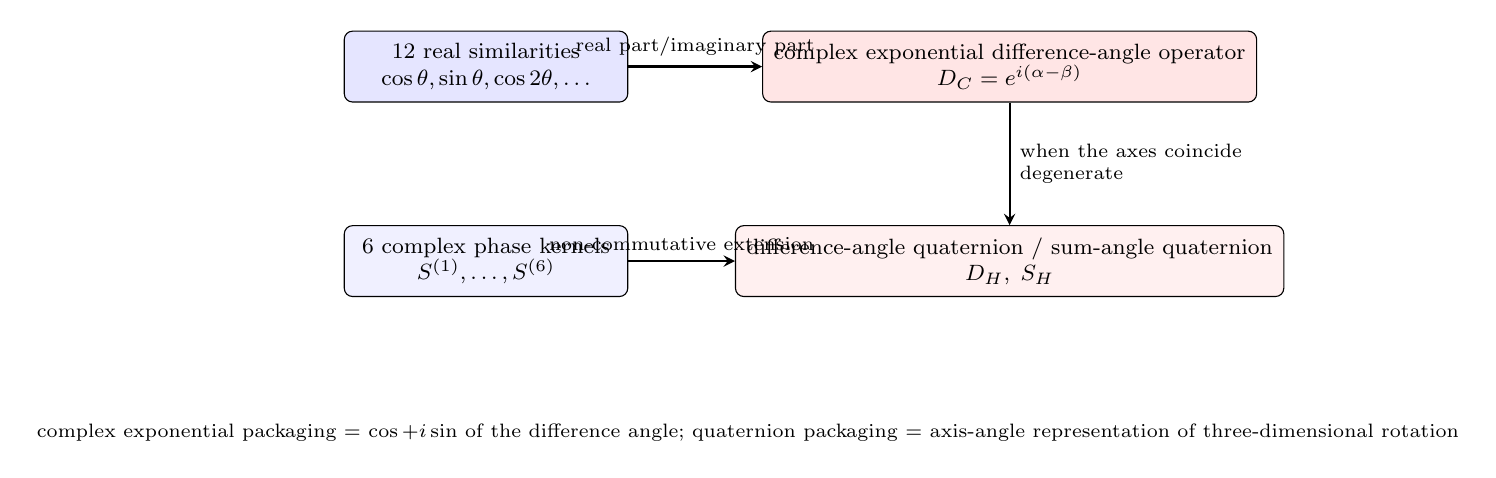
\begin{tikzpicture}[scale=0.95,>=stealth,
        box/.style={draw, rounded corners=3pt, align=center, font=\footnotesize,
                    minimum height=0.9cm, inner sep=4pt},
        arr/.style={->, thick, >=stealth}]

        \node[box, fill=blue!10, minimum width=3.6cm] (real12) at (0,2)
            {12 real similarities\\ $\cos\theta,\sin\theta,\cos 2\theta,\dots$};
        \node[box, fill=red!10, minimum width=4.2cm] (complex) at (7.0,2)
            {complex exponential difference-angle operator\\ $D_{\mathbb{C}}=e^{i(\alpha-\beta)}$};

        \node[box, fill=blue!6, minimum width=3.6cm] (real12b) at (0,-0.6)
            {6 complex phase kernels\\ $S^{(1)},\dots,S^{(6)}$};
        \node[box, fill=red!6, minimum width=4.2cm] (quat) at (7.0,-0.6)
            {difference-angle quaternion / sum-angle quaternion\\ $D_{\mathbb{H}},\;S_{\mathbb{H}}$};

        \draw[arr] (real12.east) -- node[above, font=\scriptsize] {real part/imaginary part} (complex.west);
        \draw[arr] (real12b.east) -- node[above, font=\scriptsize] {non-commutative extension} (quat.west);

        \draw[arr] (complex.south) -- node[right, font=\scriptsize, align=left]
            {when the axes coincide\\ degenerate} (quat.north);

        \node[font=\scriptsize, align=center, below=0.8cm] at (3.5,-1.8)
            {complex exponential packaging = $\cos+i\sin$ of the difference angle; quaternion packaging = axis-angle representation of three-dimensional rotation};
    \end{tikzpicture}
    \caption{The structural relation from the 12 real similarities to the complex exponential/quaternion packaging. The 6 complex phase kernels are the complex packaging of the 12 real similarities; the complex exponential difference-angle operator is the two-dimensional rotational realisation of the phase kernels; the difference-angle/sum-angle quaternions are the non-commutative extension of the same logic to three-dimensional rotations (Remark \ref{rem:exponential_similarity_relation_to_12}).}
    \label{fig:similarity_packaging}
\end{figure}

\section{\texorpdfstring{The geometric origin of the inverse-square law}{The geometric origin of the inverse-square law}}

\begin{theorem}[The geometric derivation of the inverse-square law]\label{thm:inverse_square}
Let $\mathbf{F}$ be a radial vector field centred at $O$, sourceless outside $O$, such that the magnitude of $\mathbf{F}$ depends only on the distance $r$ from $O$ (spherical symmetry). If the total flux of $\mathbf{F}$ through any closed surface enclosing $O$ is the constant $\Phi_0$, then the magnitude of $\mathbf{F}$ must be inversely proportional to the square of the distance:
\[F(r) = \frac{\Phi_0}{4\pi r^2}.\]
\end{theorem}

\begin{proof}
Take the sphere $S_r$ enclosing $O$ (of radius $r$). By hypothesis the magnitude of $\mathbf{F}$ depends only on $r$, so $F(r)$ is constant on the sphere of radius $r$; the direction is everywhere radial, so $\mathbf{F}$ is everywhere parallel to the outward normal $\mathbf{n} = \frac{\mathbf{r}}{r}$ of the surface element. The total flux through the sphere is:
\[\Phi_0 = \oiint_{S_r} \mathbf{F} \cdot d\mathbf{S} = \oiint_{S_r} F(r) \, dS = F(r) \oiint_{S_r} dS = F(r) \cdot 4\pi r^2.\]
Solving gives $F(r) = \Phi_0/(4\pi r^2)$. Hence $F(r) \propto 1/r^2$.
\end{proof}

\begin{corollary}[Inverse-square decay and conservation of flux (one-directional implications)]\label{cor:inverse_square_converse}
The converse of Theorem \ref{thm:inverse_square} holds on spheres: if a radial vector field centred at $O$ decays as
\[\mathbf{F}(\mathbf{r}) = \frac{C}{r^2} \frac{\mathbf{r}}{r}\]
then its flux through any sphere centred at $O$ is constantly equal to $4\pi C$. Moreover, the field $\mathbf F=C\mathbf r/r^3$ of the same form is sourceless for $r>0$ ($\nabla\cdot\mathbf F=0$), so by the divergence theorem its flux through any closed surface enclosing $O$ is likewise constantly $4\pi C$.
\end{corollary}

\begin{proof}
For the sphere $S_r$ centred at $O$ with radius $r$,
\[\oiint_{S_r} \mathbf{F} \cdot d\mathbf{S} = \oiint_{S_r} \frac{C}{r^2} \, dS = \frac{C}{r^2} \oiint_{S_r} dS = \frac{C}{r^2} \cdot 4\pi r^2 = 4\pi C,\]
the result being independent of $r$, hence the flux through spheres is conserved. For an arbitrary closed surface $\Sigma$ enclosing $O$, apply the divergence theorem to $\mathbf F$ on the region $\mathbb{R}^3\setminus\{O\}$ (where $\nabla\cdot\mathbf F=\frac{1}{r^2}\frac{d}{dr}\bigl(r^2\cdot\frac{C}{r^2}\bigr)=0$ for $r>0$): the flux through $\Sigma$ equals that through a concentric sphere $S_r$, hence is also $4\pi C$.
\end{proof}

\begin{remark}[`Conservation of flux' and `inverse-square decay' are not unconditionally equivalent]\label{rem:inverse_square_converse_scope}
Theorem \ref{thm:inverse_square} and Corollary \ref{cor:inverse_square_converse} together yield the following two \emph{one-directional} implications, not the biconditional `conservation of flux $\iff$ inverse-square decay':
\begin{enumerate}[label=(\roman*)]
    \item \textbf{(Sufficiency)} if $\mathbf{F}=C\mathbf{r}/r^3$, then $\mathbf F$ is sourceless for $r>0$ and the flux through any closed surface enclosing $O$ is constantly $4\pi C$;
    \item \textbf{(Necessity)} if the radial field $\mathbf{F}=F(r)\hat{\mathbf{r}}$ has constant flux $\Phi_0$ through every sphere centred at $O$, then $F(r)=\Phi_0/(4\pi r^2)$; here $\nabla\cdot\mathbf F=0$ (for $r>0$) follows from the conclusion and need not be assumed.
\end{enumerate}
The phrase `mutually necessary and sufficient conditions' must therefore be narrowed: the hypothesis of Theorem \ref{thm:inverse_square} is that the flux through every \emph{closed surface} enclosing $O$ is constant, whereas (ii) puts only spheres into the hypothesis, so the two hypotheses are not symmetric, and in (ii) the absence of sources is a consequence of the conclusion rather than a premise. Once the hypotheses are removed the equivalence fails---the field $\mathbf F=f(r)\hat{\mathbf r}$ with $f(r)=1/r^2+1$ ($r>1$) is sourceless in the region $r>1$ and spherically symmetric, yet its flux through spheres $\Phi(r)=4\pi(1+r^2)$ varies with $r$, so it is a \textbf{counterexample} to Theorem \ref{thm:inverse_square} (non-constant flux and a decay that is not purely $r^{-2}$); see \cref{ex:inverse_square_needs_const_flux} of the chapter `Vector Analysis'.
\end{remark}

\begin{example}[Newton's law of universal gravitation]
Place a mass $M$ at the source $O$; the flux of the gravitational field $\mathbf{g}$ through a closed surface enclosing $M$ is $\Phi_0 = -4\pi GM$. Here the flux is negative because the direction of the gravitational field is by convention taken to point towards the source (opposite to the outward radial direction). Substituting into Theorem \ref{thm:inverse_square} gives:
\[\mathbf{g}(\mathbf{r}) = -G \frac{M}{r^2} \cdot \frac{\mathbf{r}}{r}.\]
\end{example}

\begin{example}[Coulomb's law]
Place a charge $Q$ at the source $O$; the flux of the electric field $\mathbf{E}$ through a closed surface enclosing $Q$ is $\Phi_0 = Q/\varepsilon_0$. Substituting into Theorem \ref{thm:inverse_square} gives:
\[\mathbf{E}(\mathbf{r}) = \frac{1}{4\pi\varepsilon_0} \frac{Q}{r^2} \cdot \frac{\mathbf{r}}{r}.\]
\end{example}

\begin{remark}[The inverse-square law and the three symmetry centres]\label{rem:inverse_square_three_symmetries}
The inverse-square law embodies the concerted action of the three symmetry centres:
\begin{enumerate}[label=(\roman*)]
    \item \textbf{Rotational symmetry ($i$-symmetry)}: the source point $O$ possesses rotational symmetry of the whole space---on any sphere centred at $O$, the magnitude of the field is everywhere equal.
    \item \textbf{Proportional symmetry ($1$-symmetry)}: the field decays as $1/r^2$, that is, for each doubling of the distance the magnitude of the field shrinks to $1/4$ of its former value.
    \item \textbf{Additive reflection symmetry ($0$-symmetry)}: along any straight line through the source point $O$, the radial direction of the field exhibits reflection symmetry.
\end{enumerate}
\end{remark}

\section{\texorpdfstring{Complete correspondence table between the three symmetry centres and vector operations}{Complete correspondence table between the three symmetry centres and vector operations}}

\begin{table}[htbp]
    \centering
    \caption{The complete correspondence between the three basic generating transformations, the vector operations and the symmetry centres}
    \label{tab:symmetry_correspondence}
    \renewcommand{\arraystretch}{1.35}
    \begin{tabular}{>{\centering\arraybackslash}p{2.5cm}>{\centering\arraybackslash}p{2.5cm}>{\centering\arraybackslash}p{4.5cm}>{\centering\arraybackslash}p{3cm}}
        \toprule
        Symmetry centre and symmetry type & Basic transformation & Vector operation & Conserved quantity \\
        \midrule
        \textbf{0} (additive reflection symmetry) & Translation & vector addition $\mathbf{u}+\mathbf{v}$ & momentum \\[4pt]
         &  & vector subtraction $\mathbf{u}-\mathbf{v}$ &  \\[4pt]
         &  & inner product $\mathbf{a}\cdot\mathbf{b}$ &  \\[4pt]
         &  & reflection &  \\
        \midrule
        \textbf{1} ($c \neq 1$, multiplicative scaling reflection symmetry) & Scaling & scalar multiplication $\alpha\mathbf{u}$ & phase-space volume \\[4pt]
         &  & refraction (scaling of the sine tendency) &  \\[4pt]
         &  & scaling of the modulus &  \\
        \midrule
        \textbf{1} ($c=1$) / \textbf{i} (multiplicative inversion/$i$-symmetry) & Rotation & outer product $\mathbf{a}\times\mathbf{b}$ & angular momentum \\[4pt]
         &  & complex multiplication $z_1 z_2$ &  \\[4pt]
         &  & quaternion multiplication &  \\[4pt]
         &  & complex exponential similarity, difference-angle quaternion, sum-angle quaternion &  \\
        \bottomrule
    \end{tabular}
\end{table}

\begin{figure}[htbp]
\centering
\begin{tikzpicture}[>=stealth,
    symmetry/.style={draw, rounded corners, minimum width=2.8cm, minimum height=1.4cm, align=center, font=\small\bfseries},
    arrow/.style={->, thick, >=stealth}]

    \node[symmetry, fill=blue!10] (add) at (0,0) {additive reflection symmetry\\symmetry centre $c=0$};
    \node[symmetry, fill=red!10] (mul) at (0,-3.5) {multiplicative scaling reflection symmetry\\symmetry centre $c \neq 1$};
    \node[symmetry, fill=green!10] (rot) at (0,-7.0) {multiplicative inversion/$i$-symmetry\\symmetry centre $c=1,i$};

    \node[font=\small, right=0.3cm of add] {vector addition/subtraction, inner product, reflection};
    \node[font=\small, right=0.3cm of mul] {scalar multiplication, refraction, tendency scaling};
    \node[font=\small, right=0.3cm of rot] {outer product, complex multiplication, quaternion multiplication, exponential similarity};

    \draw[arrow, blue] (add) to[bend left=20] node[right, font=\footnotesize] {logarithmic conversion} (mul);
    \draw[arrow, red] (mul) to[bend left=20] node[left, font=\footnotesize] {exponential conversion} (add);
    \draw[arrow, orange!80!black, dashed] (mul) to[bend left=20] node[right, font=\footnotesize] {unit-circle restriction $|\lambda|=1$} (rot);
    \draw[arrow, green!60!black] (rot.west) to[bend left=30] node[left=0.6cm, font=\footnotesize] {projection} (add.west);
\end{tikzpicture}
\caption{The correspondence between the three symmetry centres and the vector operations. Additive reflection symmetry ($c=0$) corresponds to vector addition/subtraction, the inner product and reflection; multiplicative scaling reflection symmetry ($c\neq 1$) corresponds to scalar multiplication, refraction and tendency scaling; multiplicative inversion/$i$-symmetry ($c=1,i$) corresponds to the outer product, complex multiplication, quaternion multiplication, the complex exponential similarity and the difference-angle/sum-angle quaternions. The logarithmic/exponential maps realise the conversion between additive reflection symmetry and multiplicative scaling reflection symmetry, whilst the unit-circle restriction ($|\lambda|=1$) realises the hierarchical progression from multiplicative scaling reflection symmetry to multiplicative inversion symmetry.}
\label{fig:three_symmetries_correspondence}
\end{figure}

\begin{remark}[The conservation and closure themes of this chapter]\label{rem:conservation_closure_theme_ch3}
The conservation theme of this chapter consists of three groups of invariances: the cosine tendency (inner product) is conserved under the orthogonal group $O(n)$ (Proposition \ref{prop:cosine_scalar}), the absolute value of the sine tendency (the modulus of the outer product) is conserved under pure rotations $SO(3)$ (Proposition \ref{prop:sine_rotation}), and reflection preserves the modulus (Definition \ref{def:reflection_vector}) whilst refraction preserves the sine tendency along the interface normal (Definition \ref{def:refraction_vector}); the flux of a sourceless radial field is conserved on a closed surface (Theorem \ref{thm:inverse_square} and Corollary \ref{cor:inverse_square_converse}). The closure theme is borne jointly by the $2$-periodic closed orbit given by the reflection involution (Definition \ref{def:reflection_vector}) and by the flux criterion on a closed surface. These conserved quantities and closure criteria are the concrete manifestation, at the level of vector operations, of the three conservation laws of the `Operations and Periodicity' chapter (momentum, angular momentum, phase-space volume).
\end{remark}

\section{Involutions and period two: the periodic structure of discrete symmetry}
\label{sec:involution_two_period}

The correspondence established in this chapter between the three symmetry centres and the vector operations has a direct and rigorous periodic consequence: \textbf{an involution without fixed points gives a closed orbit of period exactly $2$}. This is at once the interface of this chapter with the `periodicity' theme of the whole book, and the first instance at the vector level of the smallest non-trivial period.

\begin{proposition}[Involutions induce closed orbits of period 2]\label{prop:involution_two_period}
Let $\sigma:X\to X$ satisfy $\sigma^2=\operatorname{id}$ and have no fixed point on $X$. Then for every $x\in X$ the orbit
\[
\mathcal{O}_x=\{x,\ \sigma(x)\}
\]
contains exactly two elements, and the restriction of $\sigma$ to $\mathcal{O}_x$ is a $2$-cycle; that is, every orbit of $\sigma$ is a closed orbit of least positive period $2$.
\end{proposition}

\begin{proof}
From $\sigma^2=\operatorname{id}$ we get $\sigma(\sigma(x))=x$, so $\mathcal{O}_x=\{x,\sigma(x)\}$ is closed under $\sigma$. Moreover, the absence of fixed points implies $\sigma(x)\neq x$, so $\mathcal{O}_x$ contains exactly two elements. Hence $\sigma^2(x)=x$ whilst $\sigma(x)\neq x$, and the least positive period is $2$.
\end{proof}

\begin{corollary}[Both symmetry centres of this chapter yield period 2]\label{cor:reflection_two_period}
Among the generating transformations of this chapter:
\begin{enumerate}[label=(\roman*)]
    \item \textbf{Additive reflection} $\mathbf{v}\mapsto-\mathbf{v}$ has no fixed point on $\mathbb{R}^n\setminus\{\mathbf{0}\}$, and hence gives a $2$-periodic closed orbit; its symmetry centre is $c=0$.
    \item \textbf{Multiplicative inversion} $z\mapsto z^{-1}$ has no fixed point on $\mathbb{C}\setminus\{0,1,-1\}$ (since $z^{-1}=z\iff z=\pm1$), and likewise gives a $2$-periodic closed orbit; its symmetry centre is $c=i$.
\end{enumerate}
Together the two show that \textbf{strict periodicity need not come from continuous rotation, and a discrete involution likewise produces periodicity}, except that it can give only the smallest possible non-trivial period $2$.
\end{corollary}

\begin{proof}
(i) $-\mathbf{v}=\mathbf{v}\iff\mathbf{v}=\mathbf{0}$, so there is no fixed point on $\mathbb{R}^n\setminus\{\mathbf{0}\}$, and Proposition \ref{prop:involution_two_period} gives period $2$.
(ii) Likewise, $z^{-1}=z\iff z^2=1\iff z=\pm1$.
\end{proof}

\begin{remark}[Interface with the theme of `periodicity']\label{rem:vector_two_period_interface}
Proposition \ref{prop:involution_two_period} gives the entry point of this chapter into the `periodicity' theme: \textbf{the involution} is the simplest periodic mechanism after the three continuous transformations, and the period it produces can only be $2$---this is precisely the simplest non-trivial case of order $2$ in `finite-order action $\Rightarrow$ closed orbit' of the `Operations and Periodicity' chapter. Thereby the three symmetry centres of this chapter acquire a unified interpretation at the level of periodicity:
\[
c=0\ (\text{additive reflection}),\qquad c=i\ (\text{multiplicative inversion})\ \Longrightarrow\ \text{2-periodic closed orbit}.
\]
As to why $c=1$ (scaling) does not produce a closed orbit: the continuous scaling group $(\mathbb{R}^+,\times)$ is \textbf{torsion-free}, having no non-trivial element of finite order (see \cref{cor:rotation_unique} of the `Operations and Periodicity' chapter).
\end{remark}


\section*{Seven-theme comparison table for this chapter}

\begin{center}
\begin{tabular}{>{\centering\arraybackslash}p{2.2cm}>{\centering\arraybackslash}p{9.5cm}}
\toprule
Theme & Corresponding content in this chapter \\
\midrule
Translation & Vector addition $\mathbf{u}+\mathbf{v}$ (Definition \ref{def:vector_addition_translation}) forms a commutative group (Proposition \ref{prop:vector_additive_group}); the modulus of the vector sum $\mathbf{a}+\mathbf{b}$ is the half-angle cosine tendency (Proposition \ref{prop:sum_difference_half_angle}). \\
Scaling & The modulus scaling of scalar multiplication $\alpha\mathbf{u}$ (Definition \ref{def:scalar_multiplication_scaling}); the inverse-square law $F(r)\propto r^{-2}$ (Theorem \ref{thm:inverse_square}) and Corollary \ref{cor:inverse_square_converse}. \\
Rotation & Complex multiplication adds the arguments and multiplies the moduli (Proposition \ref{prop:complex_multiplication}); quaternion multiplication realises the composition of three-dimensional rotations (Proposition \ref{prop:quaternion_multiplication}); the difference-angle quaternion as three-dimensional rotation-difference operator (Proposition \ref{prop:quaternion_exp_similarity_rotation_operator}); the sum-angle quaternion as three-dimensional rotational composition operator (Theorem \ref{thm:quaternion_sum_rotation_operator}). \\
Conservation & The cosine tendency (inner product) is invariant under $O(n)$ (Proposition \ref{prop:cosine_scalar}); the absolute value of the sine tendency (the modulus of the outer product) is invariant under $SO(3)$ (Proposition \ref{prop:sine_rotation}); reflection preserves the modulus, and refraction preserves the sine tendency along the interface normal (Definition \ref{def:reflection_vector}, \ref{def:refraction_vector}). \\
Symmetry & The reflection involution embodies additive reflection symmetry $c=0$ (Definition \ref{def:reflection_vector}); refraction scaling embodies the modulation of $i$-symmetry by multiplicative scaling reflection symmetry $c\neq 1$ (Definition \ref{def:refraction_vector}); the difference-angle quaternion is invariant under right multiplication and undergoes a conjugation transformation under left multiplication (Remark \ref{rem:quaternion_exp_similarity_noncommutative}). \\
Closure & Two reflections return to the original, $\mathbf{v}''=\mathbf{v}$, forming a closed orbit of period $2$ (Definition \ref{def:reflection_vector}); the inverse-square law takes the conservation of flux on a closed surface as its criterion (Theorem \ref{thm:inverse_square}, Corollary \ref{cor:inverse_square_converse}). \\
Period & In complex multiplication the addition of arguments makes the rotation angle compose with period $2\pi$ (Proposition \ref{prop:complex_multiplication}); the $2$-periodic closed orbit of reflection is the smallest periodic structure of this chapter (Definition \ref{def:reflection_vector}); the composition law of the difference-angle quaternion is closed (Proposition \ref{prop:quaternion_exp_similarity_composition}); when the axes coincide the quaternion case degenerates to the angle difference and angle sum of the complex case (Theorem \ref{thm:quaternion_sum_rotation_degeneration}). \\
\bottomrule
\end{tabular}
\end{center}

\section*{Exercises}

\begin{enumerate}[leftmargin=3em, label=\textbf{Exercise \arabic*}]
    \item According to Definition \ref{def:scalar} and Definition \ref{def:vector}, explain that the essential difference between a scalar and a vector lies not in `whether it carries a direction',
    but in the \textbf{transformation law under a group representation}. Give two concrete examples: a scalar field and a vector field,
    and verify that their transformation behaviour under a spatial rotation is indeed different.

    \item Prove Proposition \ref{prop:vector_additive_group}: $\mathbb{R}^n$ forms a commutative group under vector addition,
    with the zero vector as identity element and the negative vector as inverse element. Further explain that the additive reflection
    $\sigma_{\mathbf{0}}(\mathbf{u})=-\mathbf{u}$ is an involution automorphism with $\mathbf{0}$ as its unique fixed point,
    and point out that the group it generates is isomorphic to $C_2$.

    \item Verify the Cartesian-product generation in Lemma \ref{lem:similarity_generation}:
    \[
    12=\{\text{difference angle},\text{sum angle}\}\times\{\text{basic},\text{double angle},\text{half angle}\}\times\{\cos,\sin\}.
    \]
    Write down respectively the explicit expressions of the six cosine similarities and the six sine similarities
    corresponding to basic difference angle, double-angle difference angle, half-angle difference angle, basic sum angle, double-angle sum angle and half-angle sum angle
    (see Definitions \ref{def:basic_diff_similarity} to \ref{def:half_sum_similarity}).

    \item Take $\mathbf{a}=(3,4)$, $\mathbf{b}=(1,\sqrt{3})$ and compute:
    \begin{enumerate}[label=(\roman*)]
        \item the arguments $\alpha$ and $\beta$ of the two vectors;
        \item the signed difference angle $\alpha-\beta$ and the sum angle $\phi=\alpha+\beta$;
        \item the concrete numerical values of the \textbf{basic difference-angle cosine}, the \textbf{basic difference-angle sine},
              the \textbf{basic sum-angle cosine} and the \textbf{basic sum-angle sine} among the 12 similarities;
        \item the tendency values among the 12 tendencies corresponding to the above four similarities (the product of the moduli $\|\mathbf{a}\|\|\mathbf{b}\|$ times the similarity).
    \end{enumerate}
    And verify $(\operatorname{cosine})^2+(\operatorname{sine})^2=1$.

    \item Prove Proposition \ref{prop:sum_difference_half_angle}:
    when $\|\mathbf{a}\|=\|\mathbf{b}\|=r$ and the included angle is $\theta$,
    \[
    \|\mathbf{a}+\mathbf{b}\|=2r\cos\frac{\theta}{2},\qquad
    \|\mathbf{a}-\mathbf{b}\|=2r\sin\frac{\theta}{2}.
    \]
    Then explain: if the equal-modulus condition is removed, how should the formulae be corrected? Why can they not then be simplified to a single half-angle trigonometric form
    (see Remark \ref{rem:sum_difference_non_equal_length})?

    \item Verify the reflection transformation in Definition \ref{def:reflection_vector}:
    \[
    \mathbf{v}'=\mathbf{v}-2(\mathbf{v}\cdot\mathbf{n})\mathbf{n}
    \]
    is an involution ($\mathbf{v}''=\mathbf{v}$) and preserves the modulus ($\|\mathbf{v}'\|=\|\mathbf{v}\|$).
    Further prove that the double-angle cosine similarity of the direction with the normal is conserved before and after reflection, that is,
    $\cos 2\theta_{\text{in}}=\cos 2\theta_{\text{out}}$.
    Finally explain why reflection gives the smallest periodic structure of this chapter---a closed orbit of period $2$.

    \item Prove the critical-angle conclusion for Snell's law (Proposition \ref{prop:critical_angle}):
    when $n_1>n_2$ and the angle of incidence $\theta_1>\theta_c=\arcsin(n_2/n_1)$,
    Snell's law requires $\sin\theta_2>1$, which has no solution in the real domain, and total internal reflection occurs.
    Give a concrete numerical example and compute the critical angle.

    \item Prove that the complex exponential difference-angle operator
    \[
    D_{\mathbb{C}}(z_1,z_2)=\frac{z_1\overline{z_2}}{|z_1||z_2|}
    \]
    is a two-dimensional rotation-difference operator, that is,
    \[
    D_{\mathbb{C}}(z_1,z_2)\cdot\frac{z_2}{|z_2|}=\frac{z_1}{|z_1|}
    \]
    (Proposition \ref{prop:complex_exp_similarity_rotation_operator}).
    And verify the composition law
    \[
    D_{\mathbb{C}}(z_1,z_2)D_{\mathbb{C}}(z_2,z_3)=D_{\mathbb{C}}(z_1,z_3).
    \]

    \item According to Definition \ref{def:quaternion_diff_sum}, write down the explicit expressions of the difference-angle quaternion
    $D_{\mathbb{H}}(p,q)=p\overline{q}/(|p||q|)$ and the sum-angle quaternion
    $S_{\mathbb{H}}(p,q)=pq/(|p||q|)$.
    Prove that when $p,q$ have the same rotation axis ($\mathbf{u}=\mathbf{v}$),
    the difference-angle quaternion and the sum-angle quaternion degenerate respectively to
    \[
    e^{\mathbf{u}(\alpha-\beta)},\qquad e^{\mathbf{u}(\alpha+\beta)},
    \]
    completely parallel to the complex case (Theorem \ref{thm:quaternion_sum_rotation_degeneration}).

    \item Prove Theorem \ref{thm:quaternion_exp_tendency_geometry}:
    for $p=p_0+\mathbf{p}$ and $q=q_0+\mathbf{q}$, the quaternion exponential tendency
    $\operatorname{Tendency}^{\mathbb{H}}(p,q)=p\overline{q}$ satisfies
    \[
    \operatorname{Sc}(p\overline{q})=p_0q_0+\mathbf{p}\cdot\mathbf{q},
    \]
    and when $p,q$ are pure imaginary quaternions,
    \[
    \operatorname{Vec}(p\overline{q})=-\mathbf{p}\times\mathbf{q}.
    \]
    Use the quaternion multiplication formula
    $(a+\mathbf{A})(b+\mathbf{B})=ab-\mathbf{A}\cdot\mathbf{B}+a\mathbf{B}+b\mathbf{A}+\mathbf{A}\times\mathbf{B}$
    to complete the proof.

    \item Prove Theorem \ref{thm:inverse_square}:
    let $\mathbf{F}$ be a radial vector field centred at $O$, sourceless outside $O$,
    such that the magnitude of $F$ depends only on the distance $r$, and whose total flux through any closed surface enclosing $O$ is the constant $\Phi_0$.
    Then $F(r)=\Phi_0/(4\pi r^2)$.
    Then prove its converse (Corollary \ref{cor:inverse_square_converse}):
    if the radial field decays as $C/r^2$, then its flux through any sphere centred at $O$ is constantly $4\pi C$.

    \item Verify Proposition \ref{prop:cosine_scalar} and Proposition \ref{prop:sine_rotation}:
    the cosine tendency (inner product) is invariant under the orthogonal group $O(n)$;
    the absolute value of the sine tendency (the modulus of the outer product) is invariant under pure rotations $SO(3)$.
    Prove each by matrix computation, and explain that these two conservation laws correspond respectively to the conservation of the projection measure along the `translation direction' and along the `rotation direction'.

    \item Comprehensive question: according to Table \ref{tab:symmetry_correspondence} and Remark \ref{rem:conservation_closure_theme_ch3},
    explain why this chapter formulates the relation between the \textbf{gradient}, the \textbf{divergence} and the \textbf{curl} on the one hand
    and \textbf{translation}, \textbf{scaling} and \textbf{rotation} on the other as a `formal correspondence' rather than a strict theorem.
    Starting from the difference in level between `transformations acting on space' and `operators acting on fields',
    discuss the caution of this formulation, and point out under what additional conditions this correspondence can become a strict proposition
    (see the relevant discussion in the `Vector Analysis' chapter).
\end{enumerate}

